\section{Security Analysis}\label{sec:theory}
In this section, we formally analyze the security properties of ROBin. To model ROBin, we define the CSI of a wireless channel, $\mathbf{H}(\cdot)$ as a function of discrete-time $t$ and antenna mode $u$. Under this definition, the CSI in ROBin behaves as a function $\mathbf{H}\left(t,u(t)\right)$, where $u$ changes for each time step. We further assume that a sequence of $\mathbf{H}\left(t, u(t)\right)$s, forms a Markov chain \cite{tan2000first}, such that $\mathbf{H}\left(T, u(T)\right)$ is independent of past CSIs, $\left\{\mathbf{H}\left(t, u(t)\right)\mid t < T-1 \right\}$, given $\mathbf{H}\left(T{-}1, u(T{-}1)\right)$. To quantify the security of ROBin, we derive the conditional mutual information between Eve's receiving signal at time $T$, $\mathbf{R}_E(T)$, and the pre-blinding message, $\mathbf{D}_B(T)$, assuming Eve knows all previous CSIs between Alice and Bob, $\left\{\mathbf{H}_{AB}\left(t,u(t)\right)\mid t = 0,...,T{-}1\right\}$, and all CSIs between Alice and herself, $\left\{\mathbf{H}_{AE}\left(t,u(t)\right)\mid t = 0,...,T\right\}$ (Sec. \ref{sec:theo1}). Finally, we verify the correctness of the proposed metric and explain the insights gained from the analytical results (Sec. \ref{sec:theo2}).

\subsection{Secrecy Leakage as Conditional Mutual Information}
\label{sec:theo1}
% Secrecy capacity is a commonly used and well-studied metric in theoretical physical layer security studies. Although the results shown in the literature are important, they are rarely used for practical physical layer scheme evaluations, since most of them rely on assumptions that are hard to satisfy in practice (e.g., all the channels are known by the transmitter or all  nodes, SNR and block length go to infinity, etc.). Alternatively, perfect secrecy is a notation often considered in cryptosystems, which is defined as the ciphertext reveals no information about the plaintext. Similarly, the definition of perfect secrecy is so strict that makes it hardly being used.

% Perfect secrecy is a well-known cryptosystem model. Typically, a cryptosystem is considered to have perfect secrecy if, for any message $X$ and any ciphertext $Y$, we have $p(X|Y) = p(X)$, which indicates that the attacker learns nothing from the ciphertext. However, the definition is so strict that makes the notation rarely used in practice. Alternatively, 
% Besides, the definitions of perfect secrecy and secrecy capacity are not capable of indicating the practical PHY-layer attack schemes proposed in recent years. For example, for the practical known-plaintext attack proposed in \cite{schulz2014practical}, the eavesdropper's knowledge about the legitimate channel is crucial to attack performance, while this part of the information is not included in above two metrics. 

To quantify eavesdropper's capacity under known-plaintext attacks in a way congruence with cryptanalysis, we consider the secrecy leakage as the conditional mutual information between the Eve's receiving signal and the pre-blinding message, given Eve has full knowledge of all previous CSIs via known symbols. That is, we assume that, as $t=T$, all the previously transmitted symbols, $\mathbf{D}(t),\ t = 0,...,T{-}1$, are known to Eve, which allows Eve to compute $\mathbf{H}_{AB}(t, u(t)),\ t = 0,...,T{-}1$. 

Let $\mathcal{H}(T)$ defines a set of previous CSIs up to time T:
\begin{equation}
    \mathcal{H}(T) = \left\{\mathbf{H}\left(t,u(t)\right) \mid t = 0,...,T \right\}.
\end{equation}

Assuming $\mathcal{H}_{AE}(T)$ and $\mathcal{H}_{AB}(T-1)$ are known to Eve. The secrecy leakage is defined as a conditional mutual information:
\begin{equation}
    I\left(\mathbf{D}_B(T);\mathbf{R}_E(T)\mid\mathcal{H}_{AB}(T-1),\mathcal{H}_{AE}(T)\right)
    \label{metric1}
\end{equation}

% In particular, to consider the worst case to legitimate pairs, we consider a much stronger practical known-plaintext attack than that in \cite{schulz2014practical}. We assume that at time $t$, all the historical data from $X_1$ to $X_{t-1}$ is known to the attacker, and the known-plaintexts under any transmit filter are enough for the attacker to infer the historical CSI of channel A-B from $h_{AB}(1)$ to $h_{AB}(u-1)$ precisely. With the knowledge of her own channel and Bob's historical channel, the leakage of the system is defined as:
% \begin{equation}
%     I(X_t;Y_t|h_{AB}(1),\cdots,h_{AB}(u-1),h_{AE}(1),\cdots,h_{AE}(u-1),h_{AE}(u))
%     \label{metric1}
% \end{equation}
For simplicity, we first consider a single antenna system, in which $\mathbf{H}\left(t,u(t)\right)$ reduces to a scalar function $\mathbf{h}\left(t,u(t)\right)$. and the pre-coding filter becomes the inverse of the main channel, e.g., $F_A(T) = h_{AB}^{-1}\left(T,u(T)\right)$. Note that all derivations below also apply to MIMO system, which we will discuss later. The received signal at Eve's side is:
\begin{equation*}
\begin{split}
    \mathbf{R}_E(T) & = h_{AE}\left(T,u(T)\right) \left(h_{AB}^{-1}\left(T,u(T)\right) \mathbf{D}_B(T)\right) + \mathbf{N} \\
    & \triangleq h_{AB}^{-1}\left(T,u(T)\right)  \mathbf{D}_B(T) + \mathbf{N},
    \label{eq:yt}
\end{split}
\end{equation*}
after Eve equalizes $h_{AE}\left(T,u(T)\right)$. Omitting  $\mathbf{N}$, Eq. \eqref{metric1} expands to 
\begin{equation*}
    I\left(\mathbf{D}_B(T);h_{AB}^{-1}\left(T,u(T)\right)  \mathbf{D}_B(T) \mid \mathcal{H}_{AB}(T-1),\mathcal{H}_{AE}(T)\right)
    \label{metric2}
\end{equation*}
To simplify the equation above, consider the conditional probability of $h_{AB}\left(T, u(T)\right)$ given  $\mathcal{H}_{AB}(T-1)$. Due to the Markov property,  
\begin{equation*}
\begin{split}
& \Pr\left[h_{AB}\left(T, u(T)\right)\mid \mathcal{H}_{AB}(T-1)\right] = \\
& \ \ \ \ \Pr\left[h_{AB}\left(T, u(T) \right) \mid h_{AB}\left(T-1, u(T-1)\right)\right].
\end{split}
\end{equation*}
As for the conditional probability of $h_{AB}\left(T, u(T)\right)$ given $\mathcal{H}_{AE}(T)$. Although $h_{AB}\left(t, u(t)\right)$ and $h_{AE}\left(t, u(t)\right)$ are mostly independent, they are correlated at the same time step, since the antenna pattern is the same for $h_{AB}(u)$ and $h_{AE}(u)$, resulting
\begin{equation*}
\begin{split}
& \Pr\left[h_{AB}\left(T, u(T)\right)\mid \mathcal{H}_{AE}(T)\right] = \\
& \ \ \ \ \Pr\left[h_{AB}\left(T, u(T) \right) \mid h_{AE}\left(T, u(T)\right)\right].
\end{split}
\end{equation*}
Based on these conditions, we have the following Theorem:
\begin{theorem}
Assuming the wireless channel has the Markov property, the secrecy leakage of ROBin can be simplified as\footnote{The proof of this Theorem is in Appendix}:
% footnote{The proof of this Theorem can be found in our technical report at https://tinyurl.com/y2t4njcx}
\begin{align}
    I\left(\mathbf{D}_B(T);\mathbf{R}_E(T) \mid \right. & \left. \mathcal{H}_{AB}(T-1),\mathcal{H}_{AE}(T)\right) =  \nonumber \\
    I\left(\mathbf{D}_B(T);\mathbf{R}_E(T) \mid \right. & \left. h_{AB}\left(T-1, u(T-1)\right), \right. \nonumber \\
    & \left. h_{AE}\left(T-1, u(T-1)\right), \right. \nonumber \\
    & \left. h_{AE}\left(T, u(T)\right)\right) = \nonumber \\
    I\left(\mathbf{D}_B(T);\mathbf{R}_E(T) \mid \right. & \left. \delta \mathcal{H}_{ABE}(T)\right),
\label{eq:secrecy_leakage_simplified}
\end{align}
where
\begin{align*}
\delta \mathcal{H}_{ABE}(T) = \left\{ \right. & \left. h_{AB}\left(T-1, u(T-1)\right), \right. \\
& \left. h_{AE}\left(T-1, u(T-1)\right), \right.\\
& \left. h_{AE}\left(T, u(T)\right)\ \right\}
\end{align*}
\label{corollary2}
\end{theorem}
\vspace{-15pt}
This simplification allows us to calculate the numerical secrecy leakage when all the possible values of discretize CSI are in a small range. Next we use numerical results to show the relationship between channel correlation and privacy leakage.
% Generalized the condition above if above Markov chains can be summarized as:
% \begin{align}
%     \Pr[X(T)|X(1,\dots, u-1)]  & = \Pr[X(u)|X(u-1)] \label{eq:chain1} \\
%     \Pr[X(u)|Y(1,\dots,u)] & = \Pr[X(u)|Y(u)] 
%     \label{eq:chain2}
% \end{align}
% Based on these Markov chains, we have following corollary:
% \begin{corollary}
%     $I(D_B;W|\Xi,\Omega)=I(D_B;W|\Omega)$
% \label{corollary2}
% \end{corollary}
% The proof is in Appendix, including the MIMO case. Now instead of calculating $I(D_B;W|\Xi,\Omega)$, we can simply compute $I(D_B;W|\Omega)$.
% Therefore, Eq. \label{metric2} reduces to


% as the leakage metric, where $\Xi$ and $\Omega$ together are the CSI information Eve has until $u$-th transmitting mode:
% \begin{align*}
% \Xi&=\{h_{AB}(1, \dots, u-2),h_{AE}(1, \dots, u-2)\}\\
% \Omega&=\{h_{AB}(u-1),h_{AE}(u-1,u)\}
% \end{align*}
% To make the metric easy to follow, we consider only one message $D_B$ and abbreviate the notations above as:
% $D_B=\mathbf{D}_B(u)$, $Z=h^{-1}_{AB}(u)$, $W=h^{-1}_{AB}(u)D_B(u)=ZD_B$. And in this form, $D_B$, $Z$, and $W$ is analogous to the plaintext, key, and ciphertext in a cryptosystem, but here we use multiplication instead of modular operation.
% Then the final leakage we consider is:
% \begin{equation}
%     I(D_B;W|\Xi,\Omega)
% \end{equation}
% w.l.o.g., we discretize the CSI in the above leakage metric for numerical calculation, and denote the size of it as $|h|$. When the joint distribution of the CSI is known, the close form of the leakage can be obtained as well. However, a direct computing of current metric incurs exponential complexity since we need to characterize the values of $\Pr(D_B;W|\Xi,\Omega)$, which are $|D_B|^2|h|^{2u}$. Hence, to make the leakage tractable, we simplify it first.

% Obviously, it is complex to compute or get any insights with the current metric due to the overwhelming channel information. To make this leakage tractable, we simplify it first.

% Since wireless channels are commonly characterized by Markov models \cite{tan2000first}, we assume that the channel still forms a Markov chain when taking the effect of antennas into account. For the self-relation of a channel, e.g. channel A-B, since the antenna mode is randomly and independently selected, then only the  physical channel is dependent on the historical channel, which is independent of the channel before $u-1$ given the previous channel. Thus, the current CSI is independent of all past CSI given the previous CSI. Meaning that $ \Pr[h_{AB}(u)|h_{AB}(1, \dots, u-1)]=\Pr[h_{AB}(u)|h_{AB}(u-1)]$. And for the cross-relation between channel A-B and A-E, though they have different physical channel characteristics, the effect of the antenna to the CSI is fixed for them under the same $u$-th transmitting mode. Then the information of antenna profile  is the same for $h_{AB}(u)$ and $h_{AE}(u)$. Meaning that $\Pr[h_{AB}(u)|h_{AE}(1, \dots, u)]=\Pr[h_{AB}(u)|h_{AE}(u)]$.

% In general, the above Markov chains can be summarized as:
% \begin{align}
%     \Pr[X(u)|X(1,\dots, u-1)]  & = \Pr[X(u)|X(u-1)] \label{eq:chain1} \\
%     \Pr[X(u)|Y(1,\dots,u)] & = \Pr[X(u)|Y(u)] 
%     \label{eq:chain2}
% \end{align}
% Based on these Markov chains, we have following corollary:
% \begin{corollary}
%     $I(D_B;W|\Xi,\Omega)=I(D_B;W|\Omega)$
% \end{corollary}
% The proof is in Appendix, including the MIMO case. Now instead of calculating $I(D_B;W|\Xi,\Omega)$, we can simply compute $I(D_B;W|\Omega)$.

% \begin{figure*}[t]
% \begin{subfigure}[t]{0.22\textwidth}
% 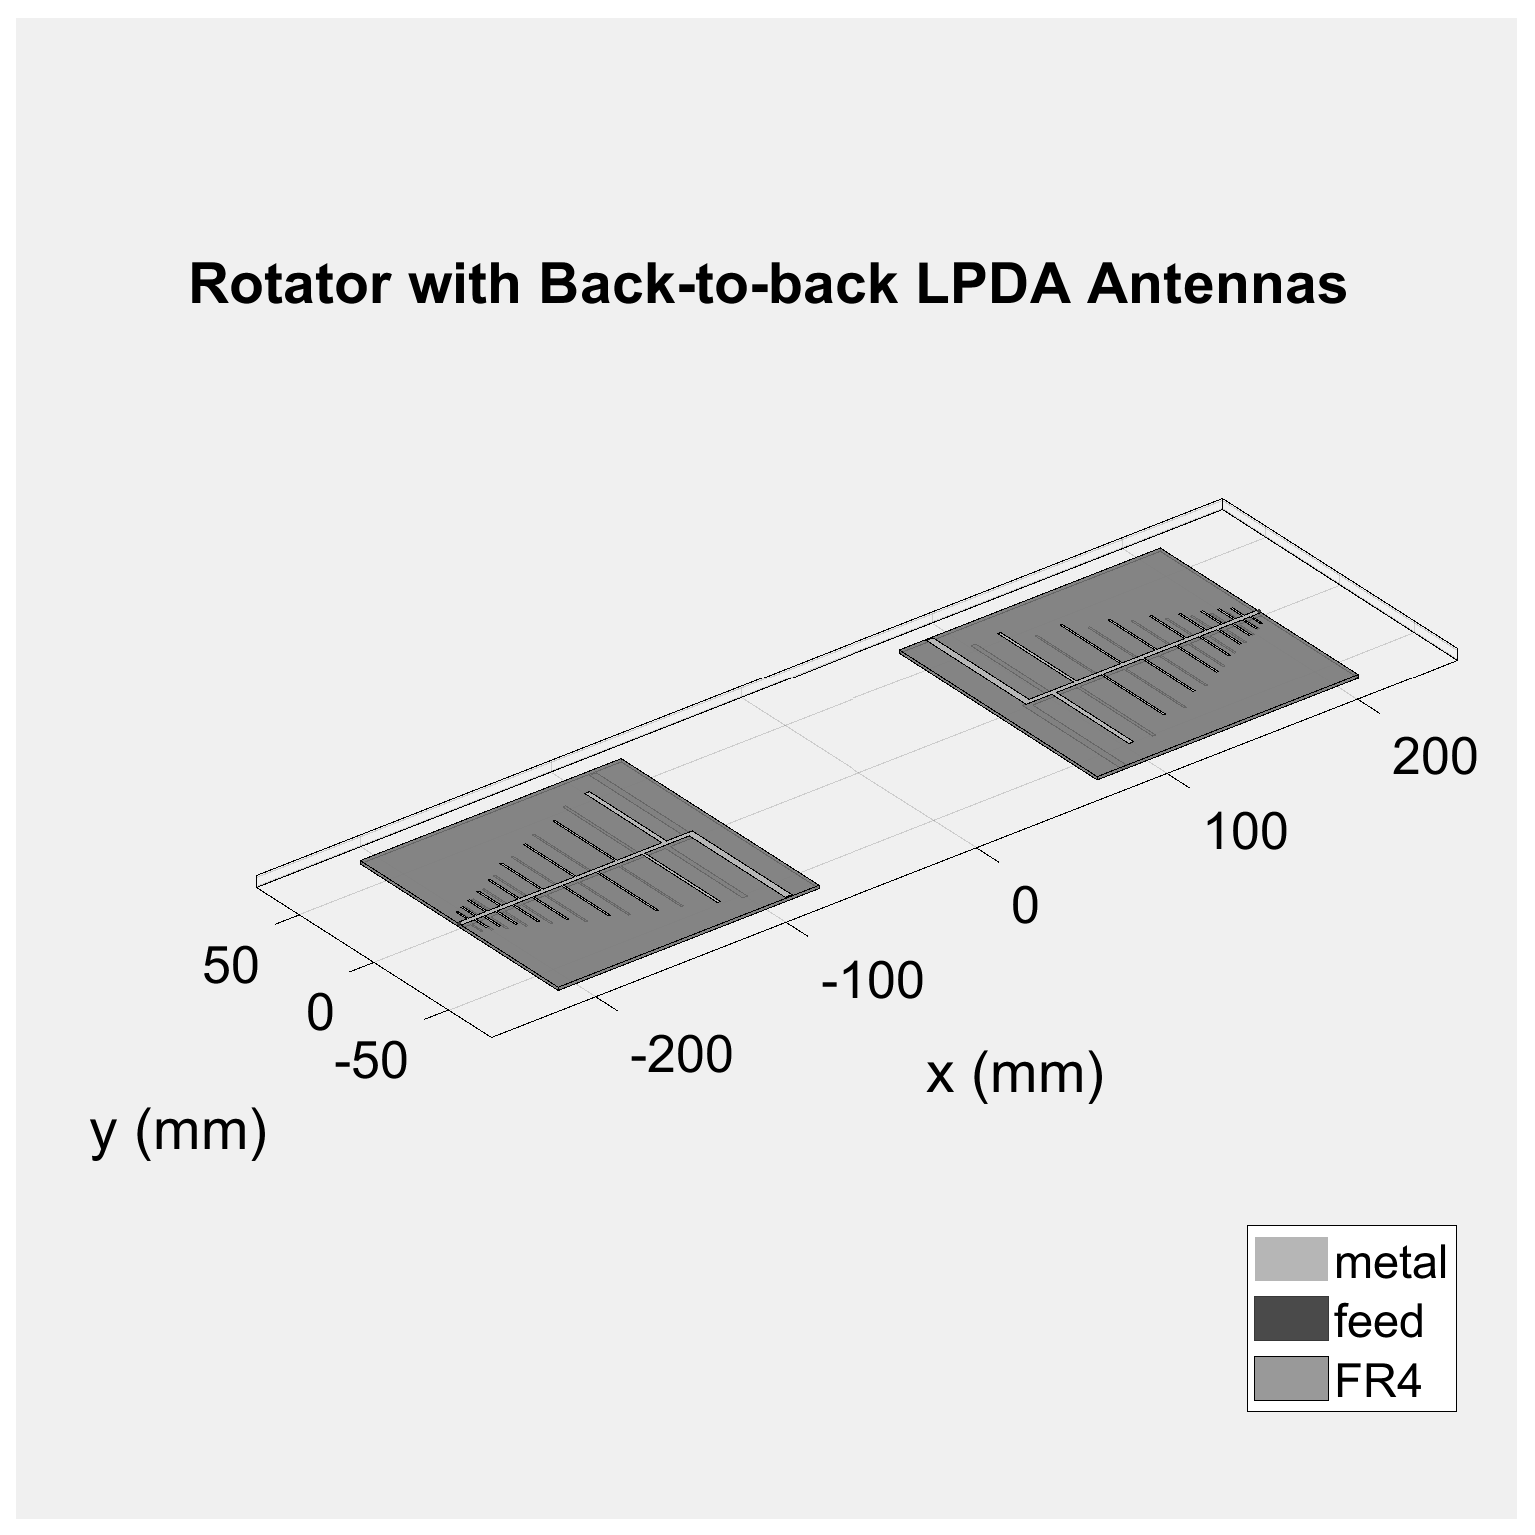
\includegraphics[width=\textwidth]{figs/rotator.eps}
% \caption{Rotator with back-to-back LPDA antennas}
% \label{fig:setup1}
% \end{subfigure}
% \hspace{\fill}
% \begin{subfigure}[t]{0.22\textwidth}
% \includegraphics[width=\textwidth]{figs/rotator_pattern.eps}
% \caption{Radiation pattern of the log periodic antenna}
% \label{wa5vjbPattern}
% \end{subfigure}
% \hspace{\fill}
% \begin{subfigure}[t]{0.22\textwidth}
% \includegraphics[width=\textwidth]{figs/testbed_02.eps}
% \caption{Our rotating reconfigurable antenna platform.}
% \label{fig:setup3}
% \end{subfigure}
% \hspace{\fill}
% \begin{subfigure}[t]{0.22\textwidth}
% \includegraphics[width=\textwidth]{figs/testbed_05.eps}
% \caption{Antenna setup for practical measurements}
% \label{fig:setup4}
% \end{subfigure}
% \vspace{-15pt}
% \end{figure*}

\subsection{Correctness and Insights}
\label{sec:theo2}
\subsubsection{Single-Antenna Eavesdropper}
Alice can apply a reduced ROBin scheme without orthogonal blinding in a single-input and single-output (SISO) system, with Bob and Eve having one regular antenna and Alice having one reconfigurable antenna. To calculate the secrecy leakage, we first generate the CSI with the truncated Gaussian distribution in the range of $(-2,2)$, then we normalize its real (imaginary) part into four values, i.e. $\text{Re}[\delta \mathcal{H}_{ABE}(T)] \in \{\pm1.5,\pm0.5\}$. And for the message we consider 4QAM, namely that $\mathbf{D}_B(T) = x \in \{\pm1 + j, \pm 1 - j\}$, then the entropy of the message is $\mathrm{H}(\mathbf{D}_B(T)) = 2$. and $\text{Re}[\mathbf{R}_E(T)] \in \{\pm1.5,\pm0.5\}$, $|\mathbf{R}_E(T)| = 16$, $|(\mathbf{D}_B(T),\mathbf{R}_E(T),\delta \mathcal{H}_{ABE}(T))| = 256 \times 2^{10}$ correspondingly. Hence we set the number of the samples to 30 million, which is about 100 times of $|(\mathbf{D}_B(T),\mathbf{R}_E(T),\delta \mathcal{H}_{ABE}(T))|$. The calculated Eq. \ref{eq:secrecy_leakage_simplified} versus correlation coefficient between $\mathbf{H}_{AB}$ and $\mathbf{H}_{AB}$ is 
shown in Fig. \ref{fig:N}.
\begin{figure}[t]
    \centering
    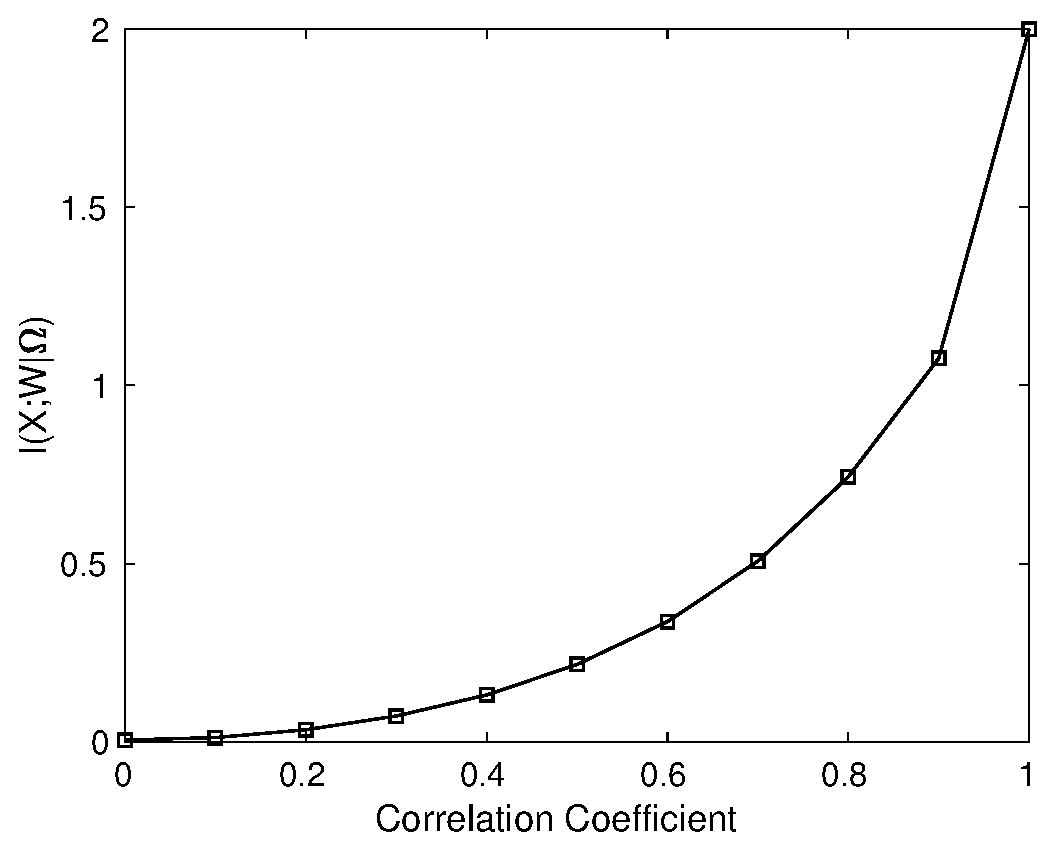
\includegraphics[width=0.25\textwidth]{figs/theory.eps}
    \caption{Secrecy leakage over the channel correlation coefficient between $\mathbf{H}_{AB}$ and $\mathbf{H}_{AB}$.}
    \label{fig:N}
    \vspace{-15pt}
\end{figure}



We can observe that the leakage increases with the increase of the correlation coefficient between $\mathbf{H}_{AB}$ and $\mathbf{H}_{AB}$, in other words, the information the eavesdropper gained decreases with the decrease of the correlation between $\mathbf{H}_{AB}$ and $\mathbf{H}_{AB}$. This result quantitatively verifies the motivation of our channel randomization strategy: the system becomes more secure after reducing the correlation between the two channels to the receiver and the eavesdropper. And results in \cite{pan2017message} shown that a reconfigurable antenna is capable of decreasing the correlation of two channels. Hence introducing a reconfigurable antenna to the system brings us two benefits: actively randomizing the wireless channel and reducing correlations among channels. 
% Besides, from the numerical results we can see that $I(X;\mathbf{W}|\Omega) \approx 0$ when correlation coefficient is 0, and $I(X;\mathbf{W}|\Omega) = H(X) = 2$ when correlation coefficient is 1, which are consistent with the lower bound and upper bound of this conditional mutual information.

%\subsubsection{MIMO System}
\subsubsection{Multi-Antenna Eavesdropper}
Alice can apply the full ROBin scheme with orthogonal blinding in a multi-input and single-output (MISO) or multi-input and multi-output (MIMO) system. Assume Eve has multiple antennas. 
For a given antenna mode, if the number of known symbols is less than the number of Alice's antennas $n_a$, Eve cannot find a unique decoding filter, because the least square problem for the LS channel estimation is underdetermined. However, the iterative decoding filter training process still provides Eve partial information about the message. And we use SER to evaluate this leakage in the simulation. When the number of known symbols is greater than $n_a$, the problem becomes overdetermined and allows Eve to identify the correct decoding filter. Nevertheless, as the number of known symbols do not accumulate when Alice reuses the same antenna mode at different channel coherent periods, as long as Alice switches the antenna mode faster than the duration of $n_a$ symbols, the secrecy leakage of our scheme is low regardless of the number of antennas Eve has.
% For a given antenna mode, if the number of known symbols is greater than the number of Alice's antennas $n_a$, the least square problem for the LS channel estimation becomes overdetermined and allows Eve to identify the correct decoding filter. When the number of known symbols is less than $n_a$, Eve cannot find a unique decoding filter, since the problem is underdetermined. However, the iterative decoding filter training process still provides Eve partial information about the message. In our simulation, we use SER to evaluate this leakage. Nevertheless, since the number of known symbols do not accumulate when Alice reuses the same antenna mode at different channel coherent periods, as long as Alice switches the antenna mode faster than the duration of $n_a$ symbols, the secrecy leakage of our scheme is low regardless of the number of antennas Eve has.

%-----------------------------------------------------------------
% \begin{figure*}[t]
% \begin{subfigure}[t]{0.24\textwidth}
% \resizebox{\columnwidth}{!}{% This file was created by matlab2tikz.
% Minimal pgfplots version: 1.3
%
%The latest updates can be retrieved from
%  http://www.mathworks.com/matlabcentral/fileexchange/22022-matlab2tikz
%where you can also make suggestions and rate matlab2tikz.
%
\begin{tikzpicture}

\begin{axis}[%
width=\tikzfigW,
height=\tikzfigH,
at={(0.758333in,0.525in)},
scale only axis,
xmin=10,
xmax=40,
xtick={10, 20, 30, 40},
xlabel={No. of training modes},
ymode=log,
ymin=1e-08,
ymax=1,
ytick={ 1e-08,  1e-06, 0.0001,   0.01,    0.1},
yminorticks=true,
ylabel={SER},
label style={font=\small},
tick label style={font=\small},
legend style={at={(0.45,0.4)},anchor=south west,legend cell align=left,align=left,draw=white!15!black,font=\scriptsize}
]
\addplot [color=black,solid,line width=1.0pt]
  table[row sep=crcr]{%
10	0.0187450086805556\\
20	0.00150703125\\
30	3.90624999999978e-07\\
40	4.34027777777778e-08\\
};
\addlegendentry{$\text{Bob}_{\text{ROBin}}$};

\addplot [color=black,solid,line width=1.0pt,mark=star,mark options={solid}]
  table[row sep=crcr]{%
10	0.0603373263888889\\
20	0.0673694444444444\\
30	0.0612369357638889\\
40	0.0602316840277778\\
};
\addlegendentry{$\text{Eve}_{\text{ROBin}}$};

\addplot [color=black,dash dot,line width=1.0pt]
  table[row sep=crcr]{%
10	4.34027777777778e-08\\
20	4.34027777777778e-08\\
30	4.34027777777778e-08\\
40	4.34027777777778e-08\\
};
\addlegendentry{$\text{Bob}$};

\addplot [color=black,dashed,line width=1.0pt]
  table[row sep=crcr]
%     \caption{SER of Bob and Eve over the number of training modes. SNR = 25dB; NDR = 1; Eve's SER is obtained after 240 iterations.}
%     \label{fig:numSamples}
% \end{subfigure}
% \hspace{\fill}
% \begin{subfigure}[t]{0.24\textwidth}
% \resizebox{\columnwidth}{!}{% This file was created by matlab2tikz.
% Minimal pgfplots version: 1.3
%
%The latest updates can be retrieved from
%  http://www.mathworks.com/matlabcentral/fileexchange/22022-matlab2tikz
%where you can also make suggestions and rate matlab2tikz.
%
\begin{tikzpicture}

\begin{axis}[%
width=\tikzfigW,
height=\tikzfigH,
at={(0.758333in,0.490972in)},
scale only axis,
xmin=1,
xmax=10,
xtick={ 1,  2,  4,  6,  8, 10},
xlabel={NDR},
ymode=log,
ymin=1e-08,
ymax=1,
ytick={ 1e-08,  1e-06, 0.0001,   0.01,      1},
yminorticks=true,
ylabel={Bob's SER},
label style={font=\small},
tick label style={font=\small},
legend style={at={(0.25,0.04)},anchor=south west,legend cell align=left,align=left,draw=white!15!black,font=\scriptsize}
]
% \addplot [color=black,dashed,line width=1.0pt]
%   table[row sep=crcr]{%
% 1	0.000986111111111111\\
% 2	0.00493433159722222\\
% 4	0.0260634548611111\\
% 6	0.0590388454861111\\
% 8	0.0982852864583333\\
% 10	0.137298567708333\\
% };
% \addlegendentry{$\text{SNR}_{\text{ROBin}}\text{=15dB}$}

% \addplot [color=black,dashed,line width=1.0pt,mark=x,mark options={solid}]
%   table[row sep=crcr]{%
% 1	0.000128602430555556\\
% 2	0.00164865451388889\\
% 4	0.00938823784722223\\
% 6	0.0204099392361111\\
% 8	0.0361276041666667\\
% 10	0.0567549479166667\\
% };
% \addlegendentry{$\text{SNR}_{\text{ROBin}}\text{=20dB}$}

\addplot [color=black,solid,line width=1.0pt]
  table[row sep=crcr]{%
1	0.000122743055555556\\
2	0.00112291666666667\\
4	0.00599483506944444\\
6	0.0107560329861111\\
8	0.0175454427083333\\
10	0.0252785590277778\\
};
\addlegendentry{$\text{SNR}_{\text{ROBin}}\text{=25dB}$}

\addplot [color=black,dashed,line width=1.0pt]
  table[row sep=crcr]{%
1	6.77083333333328e-06\\
2	0.00128888888888889\\
4	0.00580078125\\
6	0.00843862847222222\\
8	0.012955859375\\
10	0.0177450954861111\\
};
\addlegendentry{$\text{SNR}_{\text{ROBin}}\text{=30dB}$}


% \addplot [color=black,solid,line width=1.0pt]
%   table[row sep=crcr]{%
% 1	0.000699652777777778\\
% 2	0.00341688368055556\\
% 4	0.0201337239583333\\
% 6	0.0510474826388889\\
% 8	0.0879983506944444\\
% 10	0.125694965277778\\
% };
% \addlegendentry{$\text{SNR}_\text{OB}\text{=15dB}$};

% \addplot [color=black,solid,line width=1.0pt,mark=x,mark options={solid}]
%   table[row sep=crcr]{%
% 1	4.60069444444446e-05\\
% 2	0.000383159722222222\\
% 4	0.00349991319444444\\
% 6	0.01133359375\\
% 8	0.0246471788194444\\
% 10	0.0419066840277778\\
% };
% \addlegendentry{$\text{SNR}_\text{OB}\text{=20dB}$};

\addplot [color=black,dash dot,line width=1.0pt]
  table[row sep=crcr]{%
1	8.68055555555136e-08\\
2	7.20486111111118e-06\\
4	0.000420486111111111\\
6	0.00194926215277778\\
8	0.00467591145833333\\
10	0.00904301215277778\\
};
\addlegendentry{$\text{SNR}_\text{OB}\text{=25dB}$};

\addplot [color=black,solid,line width=1.0pt,mark=star,mark options={solid}]
  table[row sep=crcr]
%     \caption{SER of Bob over Alice's NDR for differnetn SNRs. Number of training modes is 20.}
%     \label{fig:SNRNDR}
% \end{subfigure}
% \hspace{\fill}
% \begin{subfigure}[t]{0.24\textwidth}
% \resizebox{\columnwidth}{!}{% This file was created by matlab2tikz.
% Minimal pgfplots version: 1.3
%
%The latest updates can be retrieved from
%  http://www.mathworks.com/matlabcentral/fileexchange/22022-matlab2tikz
%where you can also make suggestions and rate matlab2tikz.
%
\begin{tikzpicture}

\begin{axis}[%
width=\tikzfigW,
height=\tikzfigH,
%at={(0.758333in,0.490972in)},
scale only axis,
xmin=0,
xmax=250,
xlabel={Number of Iterations},
ymin=0.35,
ymax=0.75,
xtick={ 0, 50, 100, 150, 200, 250},
ytick={ 0.3, 0.45, 0.55, 0.65, 0.75},
ylabel={Eve's SER},
label style={font=\small},
tick label style={font=\small},
legend style={at={(0.4,0.35)},anchor=south west,legend cell align=left,align=left,draw=white!15!black,font=\scriptsize}
]
\addplot [color=black,double,line width=1.0pt]
  table[row sep=crcr]{%
1	0.714592881944445\\
2	0.674533854166667\\
3	0.646288194444445\\
4	0.639197048611111\\
5	0.608267795138889\\
6	0.591979166666667\\
7	0.577979166666667\\
8	0.56727734375\\
9	0.55693359375\\
10	0.548439236111111\\
11	0.53977734375\\
12	0.533875\\
13	0.526740885416667\\
14	0.523\\
15	0.517506944444444\\
16	0.508233940972222\\
17	0.498724826388889\\
18	0.493434461805556\\
19	0.491013020833333\\
20	0.487888020833333\\
21	0.483762152777778\\
22	0.483190104166667\\
23	0.481740885416667\\
24	0.47898828125\\
25	0.47512890625\\
26	0.471596354166667\\
27	0.466875434027778\\
28	0.462352864583333\\
29	0.461723958333333\\
30	0.461149305555555\\
31	0.460009548611111\\
32	0.457713541666667\\
33	0.457713541666667\\
34	0.457713541666667\\
35	0.455958767361111\\
36	0.454307291666667\\
37	0.45384375\\
38	0.453666232638889\\
39	0.449940538194444\\
40	0.449754774305556\\
41	0.447524305555556\\
42	0.446190538194444\\
43	0.446190538194444\\
44	0.4450234375\\
45	0.444446614583333\\
46	0.442932725694444\\
47	0.440263020833333\\
48	0.440263020833333\\
49	0.439627604166667\\
50	0.439627604166667\\
51	0.438510850694445\\
52	0.436240017361111\\
53	0.434579427083333\\
54	0.433573784722222\\
55	0.432697916666667\\
56	0.430939236111111\\
57	0.430607638888889\\
58	0.428844184027778\\
59	0.428799479166667\\
60	0.428799479166667\\
61	0.426791232638889\\
62	0.426525173611111\\
63	0.426102430555556\\
64	0.425759982638889\\
65	0.425759982638889\\
66	0.425759982638889\\
67	0.425759982638889\\
68	0.423932725694444\\
69	0.422850694444444\\
70	0.422567274305556\\
71	0.422567274305556\\
72	0.422539930555556\\
73	0.420638020833333\\
74	0.420637152777778\\
75	0.420635416666667\\
76	0.420328993055556\\
77	0.420328993055556\\
78	0.420328993055556\\
79	0.419638020833333\\
80	0.419638020833333\\
81	0.419092013888889\\
82	0.419075954861111\\
83	0.418581597222222\\
84	0.418415798611111\\
85	0.415895833333333\\
86	0.415387586805556\\
87	0.415358072916667\\
88	0.415009114583333\\
89	0.414886284722222\\
90	0.414879340277778\\
91	0.4145078125\\
92	0.414423177083333\\
93	0.414423177083333\\
94	0.414386284722222\\
95	0.414386284722222\\
96	0.414385850694444\\
97	0.414357638888889\\
98	0.414334201388889\\
99	0.414026041666667\\
100	0.414026041666667\\
101	0.413739149305556\\
102	0.413739149305556\\
103	0.413342013888889\\
104	0.413342013888889\\
105	0.413342013888889\\
106	0.412254340277778\\
107	0.412254340277778\\
108	0.412254340277778\\
109	0.412254340277778\\
110	0.412254340277778\\
111	0.412081597222222\\
112	0.412081163194444\\
113	0.412061631944444\\
114	0.41101171875\\
115	0.41101171875\\
116	0.410981770833333\\
117	0.409819444444444\\
118	0.409817274305556\\
119	0.409817274305556\\
120	0.409817274305556\\
121	0.409817274305556\\
122	0.409806857638889\\
123	0.409806857638889\\
124	0.409806857638889\\
125	0.409490451388889\\
126	0.409490451388889\\
127	0.409490451388889\\
128	0.408853732638889\\
129	0.408853732638889\\
130	0.408851996527778\\
131	0.408851996527778\\
132	0.408851996527778\\
133	0.408654947916667\\
134	0.408654947916667\\
135	0.408654947916667\\
136	0.40758984375\\
137	0.40758984375\\
138	0.407583767361111\\
139	0.407583767361111\\
140	0.407583767361111\\
141	0.407583767361111\\
142	0.407583767361111\\
143	0.407548611111111\\
144	0.407548611111111\\
145	0.407548611111111\\
146	0.407014322916667\\
147	0.407014322916667\\
148	0.407014322916667\\
149	0.407014322916667\\
150	0.407014322916667\\
151	0.406959635416667\\
152	0.406959635416667\\
153	0.406959635416667\\
154	0.406959635416667\\
155	0.406655381944445\\
156	0.406655381944445\\
157	0.406655381944445\\
158	0.406655381944445\\
159	0.406655381944445\\
160	0.406655381944445\\
161	0.406655381944445\\
162	0.406655381944445\\
163	0.4064921875\\
164	0.405970920138889\\
165	0.405970920138889\\
166	0.405970920138889\\
167	0.405970920138889\\
168	0.405970920138889\\
169	0.405970920138889\\
170	0.405970920138889\\
171	0.405970920138889\\
172	0.405957899305556\\
173	0.405930121527778\\
174	0.405930121527778\\
175	0.405930121527778\\
176	0.405930121527778\\
177	0.405930121527778\\
178	0.405605034722222\\
179	0.405604600694445\\
180	0.405604600694445\\
181	0.405604600694445\\
182	0.4055390625\\
183	0.405524305555556\\
184	0.405515625\\
185	0.405434461805556\\
186	0.405434461805556\\
187	0.405434461805556\\
188	0.405434027777778\\
189	0.405434027777778\\
190	0.405434027777778\\
191	0.405433159722222\\
192	0.405433159722222\\
193	0.405433159722222\\
194	0.405433159722222\\
195	0.405433159722222\\
196	0.405433159722222\\
197	0.405433159722222\\
198	0.405433159722222\\
199	0.405426215277778\\
200	0.404825086805556\\
201	0.404825086805556\\
202	0.404805555555556\\
203	0.404805555555556\\
204	0.403477864583333\\
205	0.403222222222222\\
206	0.403222222222222\\
207	0.403222222222222\\
208	0.401485677083333\\
209	0.401485677083333\\
210	0.401485677083333\\
211	0.40121875\\
212	0.40121875\\
213	0.40121875\\
214	0.40121875\\
215	0.40121875\\
216	0.40121875\\
217	0.40121875\\
218	0.401112847222222\\
219	0.401112847222222\\
220	0.401112847222222\\
221	0.401112847222222\\
222	0.400892795138889\\
223	0.400832465277778\\
224	0.400832465277778\\
225	0.400335503472222\\
226	0.400335503472222\\
227	0.400335503472222\\
228	0.400335503472222\\
229	0.400335503472222\\
230	0.400217447916667\\
231	0.400217447916667\\
232	0.400217447916667\\
233	0.400128472222222\\
234	0.400128472222222\\
235	0.399789496527778\\
236	0.399789496527778\\
237	0.399514756944445\\
238	0.399514756944445\\
239	0.399514756944445\\
240	0.399514756944445\\
};
\addlegendentry{NDR=1};

\addplot [color=black,dash dot,line width=1.0pt]
  table[row sep=crcr]{%
1	0.710848090277778\\
2	0.698789930555556\\
3	0.680871961805556\\
4	0.674679253472222\\
5	0.6576796875\\
6	0.648643663194445\\
7	0.641080729166667\\
8	0.637694010416667\\
9	0.631934461805556\\
10	0.626782552083333\\
11	0.621791232638889\\
12	0.618710503472222\\
13	0.616751736111111\\
14	0.612813802083333\\
15	0.608802951388889\\
16	0.608465711805556\\
17	0.605220486111111\\
18	0.602271701388889\\
19	0.596276475694445\\
20	0.59311328125\\
21	0.591311197916666\\
22	0.584938368055555\\
23	0.583009982638889\\
24	0.5816796875\\
25	0.577289496527778\\
26	0.576146701388889\\
27	0.572860677083333\\
28	0.570184895833334\\
29	0.568718315972222\\
30	0.564602864583334\\
31	0.563834201388889\\
32	0.56230859375\\
33	0.558663628472222\\
34	0.557739149305556\\
35	0.556705295138889\\
36	0.554381510416667\\
37	0.554180121527778\\
38	0.552649739583333\\
39	0.550235677083333\\
40	0.548788194444444\\
41	0.548545572916667\\
42	0.546330295138889\\
43	0.543867621527778\\
44	0.542759114583333\\
45	0.540443142361111\\
46	0.5403515625\\
47	0.537802083333333\\
48	0.537756076388889\\
49	0.536391059027778\\
50	0.535287760416667\\
51	0.533506944444445\\
52	0.532684461805556\\
53	0.530159722222222\\
54	0.529042534722222\\
55	0.5289140625\\
56	0.527090277777778\\
57	0.524095052083334\\
58	0.518552951388889\\
59	0.518362413194444\\
60	0.518057291666667\\
61	0.51770703125\\
62	0.516913194444445\\
63	0.516312934027778\\
64	0.516047743055556\\
65	0.514745659722222\\
66	0.514745659722222\\
67	0.512763888888889\\
68	0.512760416666667\\
69	0.512582465277778\\
70	0.512582465277778\\
71	0.51222265625\\
72	0.512204861111111\\
73	0.508993923611111\\
74	0.508806857638889\\
75	0.508566840277778\\
76	0.508377604166667\\
77	0.508377604166667\\
78	0.508375\\
79	0.50833203125\\
80	0.506624565972222\\
81	0.50651171875\\
82	0.50611328125\\
83	0.5057265625\\
84	0.505297743055556\\
85	0.503138454861111\\
86	0.503116319444444\\
87	0.501066840277778\\
88	0.4990625\\
89	0.496736979166667\\
90	0.496636284722222\\
91	0.496633680555555\\
92	0.496592447916667\\
93	0.496578559027778\\
94	0.496368923611111\\
95	0.495852864583333\\
96	0.495852864583333\\
97	0.495456163194444\\
98	0.493940104166667\\
99	0.493789496527778\\
100	0.4929765625\\
101	0.491664496527778\\
102	0.488654513888889\\
103	0.487847222222222\\
104	0.487847222222222\\
105	0.487825520833333\\
106	0.487789930555556\\
107	0.486236979166667\\
108	0.486236979166667\\
109	0.486223090277778\\
110	0.486039930555556\\
111	0.485891493055556\\
112	0.484575954861111\\
113	0.484505208333333\\
114	0.484505208333333\\
115	0.484189236111111\\
116	0.4836875\\
117	0.483649305555556\\
118	0.482748263888889\\
119	0.482662760416667\\
120	0.48226953125\\
121	0.482002170138889\\
122	0.481973958333333\\
123	0.481973958333333\\
124	0.481973958333333\\
125	0.48144921875\\
126	0.48144921875\\
127	0.481420138888889\\
128	0.480919270833333\\
129	0.48085546875\\
130	0.48085546875\\
131	0.480456597222222\\
132	0.48036328125\\
133	0.479254340277778\\
134	0.479205295138889\\
135	0.479174913194444\\
136	0.47916796875\\
137	0.479085069444444\\
138	0.47892578125\\
139	0.478852864583333\\
140	0.477772569444444\\
141	0.477772569444444\\
142	0.477772569444444\\
143	0.477384548611111\\
144	0.477097222222222\\
145	0.477021267361111\\
146	0.477021267361111\\
147	0.477021267361111\\
148	0.477020399305556\\
149	0.476991753472222\\
150	0.476991753472222\\
151	0.476991753472222\\
152	0.476962673611111\\
153	0.476634548611111\\
154	0.476634548611111\\
155	0.476611979166667\\
156	0.476478732638889\\
157	0.476307725694444\\
158	0.475995659722222\\
159	0.475946180555556\\
160	0.475900607638889\\
161	0.475318142361111\\
162	0.475270399305556\\
163	0.475270399305556\\
164	0.475270399305556\\
165	0.47519921875\\
166	0.474144965277778\\
167	0.473908854166667\\
168	0.473546006944444\\
169	0.473546006944444\\
170	0.473546006944444\\
171	0.473546006944444\\
172	0.473546006944444\\
173	0.473492621527778\\
174	0.473492621527778\\
175	0.473465711805556\\
176	0.473465711805556\\
177	0.473465711805556\\
178	0.473365885416667\\
179	0.473330295138889\\
180	0.473325954861111\\
181	0.473325954861111\\
182	0.473254774305556\\
183	0.473241319444444\\
184	0.473241319444444\\
185	0.473241319444444\\
186	0.473241319444444\\
187	0.473241319444444\\
188	0.473172743055556\\
189	0.472678819444444\\
190	0.472650607638889\\
191	0.472589409722222\\
192	0.471187065972222\\
193	0.471187065972222\\
194	0.469980034722222\\
195	0.469980034722222\\
196	0.468310763888889\\
197	0.468310763888889\\
198	0.468310763888889\\
199	0.468310763888889\\
200	0.468148871527778\\
201	0.467302951388889\\
202	0.465709201388889\\
203	0.465709201388889\\
204	0.465509548611111\\
205	0.465509548611111\\
206	0.465247395833333\\
207	0.465247395833333\\
208	0.465157118055556\\
209	0.465157118055556\\
210	0.465157118055556\\
211	0.463236979166667\\
212	0.463236979166667\\
213	0.463236979166667\\
214	0.463236979166667\\
215	0.463236979166667\\
216	0.463187065972222\\
217	0.463187065972222\\
218	0.463187065972222\\
219	0.463187065972222\\
220	0.463187065972222\\
221	0.462751736111111\\
222	0.462751736111111\\
223	0.462751736111111\\
224	0.462676649305556\\
225	0.462676649305556\\
226	0.462676649305556\\
227	0.462676649305556\\
228	0.462676649305556\\
229	0.462671440972222\\
230	0.461669270833333\\
231	0.461641059027778\\
232	0.461634114583333\\
233	0.461567708333333\\
234	0.461540798611111\\
235	0.461266059027778\\
236	0.461067708333333\\
237	0.460955295138889\\
238	0.460940538194444\\
239	0.460921006944444\\
240	0.460921006944444\\
};
\addlegendentry{NDR=2};

\addplot [color=black,dash pattern={on 7pt off 2pt on 1pt off 3pt},line width=1.0pt]
  table[row sep=crcr]{%
1	0.727302517361111\\
2	0.717838541666667\\
3	0.712375434027778\\
4	0.703504774305556\\
5	0.690833333333333\\
6	0.687000868055555\\
7	0.678313368055555\\
8	0.672259114583333\\
9	0.667538628472222\\
10	0.663371527777778\\
11	0.661121527777778\\
12	0.659459201388889\\
13	0.657967447916667\\
14	0.655009114583333\\
15	0.65425\\
16	0.649024305555556\\
17	0.646826822916667\\
18	0.646671875\\
19	0.645590277777778\\
20	0.637484375\\
21	0.635936197916667\\
22	0.633610243055556\\
23	0.631505208333333\\
24	0.630106336805556\\
25	0.625784722222222\\
26	0.62483203125\\
27	0.623167534722222\\
28	0.616668402777778\\
29	0.615658854166667\\
30	0.614338975694445\\
31	0.61403125\\
32	0.6125703125\\
33	0.61173046875\\
34	0.6108125\\
35	0.608401475694444\\
36	0.608161458333333\\
37	0.603966145833333\\
38	0.603391493055555\\
39	0.602495659722222\\
40	0.600479166666667\\
41	0.599174913194444\\
42	0.59638671875\\
43	0.59628125\\
44	0.589677951388889\\
45	0.584988715277778\\
46	0.582837673611111\\
47	0.582401475694444\\
48	0.581598958333333\\
49	0.578947482638889\\
50	0.578267361111111\\
51	0.57659765625\\
52	0.573326822916667\\
53	0.572567274305556\\
54	0.572029079861111\\
55	0.569092447916667\\
56	0.568534722222222\\
57	0.568521701388889\\
58	0.567871527777778\\
59	0.567065972222222\\
60	0.5662421875\\
61	0.565704861111111\\
62	0.564117621527778\\
63	0.564001736111111\\
64	0.561648003472222\\
65	0.561225694444444\\
66	0.561101128472222\\
67	0.560822916666667\\
68	0.559851996527778\\
69	0.558896701388889\\
70	0.557799913194444\\
71	0.554766927083333\\
72	0.554612847222222\\
73	0.5545078125\\
74	0.552812065972222\\
75	0.551641927083333\\
76	0.551446614583333\\
77	0.551417100694444\\
78	0.550857638888889\\
79	0.54856640625\\
80	0.548552517361111\\
81	0.548552517361111\\
82	0.548415798611111\\
83	0.547518663194444\\
84	0.547320746527778\\
85	0.5456015625\\
86	0.544114583333333\\
87	0.543718315972222\\
88	0.543718315972222\\
89	0.543384982638889\\
90	0.543354166666667\\
91	0.543354166666667\\
92	0.542685329861111\\
93	0.542291232638889\\
94	0.542291232638889\\
95	0.541704427083333\\
96	0.541392361111111\\
97	0.541184461805555\\
98	0.541184461805555\\
99	0.540395399305555\\
100	0.539813802083333\\
101	0.538690538194444\\
102	0.538312065972222\\
103	0.538296006944444\\
104	0.537884114583333\\
105	0.537766927083333\\
106	0.536621961805556\\
107	0.536621961805556\\
108	0.535848524305556\\
109	0.535439236111111\\
110	0.535439236111111\\
111	0.535439236111111\\
112	0.535287760416667\\
113	0.534663628472222\\
114	0.534647135416667\\
115	0.534647135416667\\
116	0.530291232638889\\
117	0.530080295138889\\
118	0.530080295138889\\
119	0.529895399305556\\
120	0.529838975694444\\
121	0.529279513888889\\
122	0.526983506944444\\
123	0.526917534722222\\
124	0.526810329861111\\
125	0.526668402777778\\
126	0.52662109375\\
127	0.52662109375\\
128	0.526598958333333\\
129	0.526335069444444\\
130	0.524943576388889\\
131	0.524927083333333\\
132	0.522205295138889\\
133	0.522193142361111\\
134	0.522189670138889\\
135	0.522157118055556\\
136	0.522115451388889\\
137	0.52210546875\\
138	0.521940972222222\\
139	0.521859375\\
140	0.521859375\\
141	0.521591145833333\\
142	0.521331163194445\\
143	0.52125390625\\
144	0.521032552083333\\
145	0.5204375\\
146	0.5204375\\
147	0.5204375\\
148	0.520275173611111\\
149	0.520275173611111\\
150	0.520200086805555\\
151	0.519489149305556\\
152	0.519065104166667\\
153	0.518360677083333\\
154	0.517512152777778\\
155	0.517458767361111\\
156	0.517458767361111\\
157	0.515874131944444\\
158	0.515450954861111\\
159	0.515450954861111\\
160	0.515384114583333\\
161	0.514747829861111\\
162	0.514663628472222\\
163	0.514663628472222\\
164	0.514640625\\
165	0.512838541666666\\
166	0.512815104166667\\
167	0.512815104166667\\
168	0.512815104166667\\
169	0.512815104166667\\
170	0.51209765625\\
171	0.51209375\\
172	0.51209375\\
173	0.51209375\\
174	0.51209375\\
175	0.512090711805555\\
176	0.511500868055555\\
177	0.511500868055555\\
178	0.511500868055555\\
179	0.511287326388889\\
180	0.510775607638889\\
181	0.510770833333333\\
182	0.510721788194444\\
183	0.510721788194444\\
184	0.510721788194444\\
185	0.510717881944444\\
186	0.510717881944444\\
187	0.510459201388889\\
188	0.510415364583333\\
189	0.510415364583333\\
190	0.510415364583333\\
191	0.510415364583333\\
192	0.510125\\
193	0.510097222222222\\
194	0.509569010416667\\
195	0.509569010416667\\
196	0.509518229166667\\
197	0.509512586805555\\
198	0.509506944444444\\
199	0.5086640625\\
200	0.50855859375\\
201	0.50786328125\\
202	0.507458333333333\\
203	0.507431423611111\\
204	0.507389322916666\\
205	0.507389322916666\\
206	0.507325086805555\\
207	0.5070546875\\
208	0.506970486111111\\
209	0.506571614583333\\
210	0.506052083333333\\
211	0.504655381944444\\
212	0.504522569444444\\
213	0.50358984375\\
214	0.50358984375\\
215	0.503589409722222\\
216	0.503589409722222\\
217	0.503588107638889\\
218	0.503588107638889\\
219	0.503583767361111\\
220	0.503578993055555\\
221	0.503578993055555\\
222	0.503560329861111\\
223	0.502473958333333\\
224	0.502458333333333\\
225	0.502194444444444\\
226	0.502153211805555\\
227	0.50213671875\\
228	0.50213671875\\
229	0.50213671875\\
230	0.501815538194444\\
231	0.500952256944444\\
232	0.500507378472222\\
233	0.500442708333333\\
234	0.500143663194444\\
235	0.500017795138889\\
236	0.49970703125\\
237	0.49793359375\\
238	0.497933159722222\\
239	0.497930121527778\\
240	0.497930121527778\\
};
\addlegendentry{NDR=4};

\addplot [color=black,densely dotted,line width=1.0pt]
  table[row sep=crcr]{%
1	0.736930989583333\\
2	0.728983940972222\\
3	0.723530815972222\\
4	0.720104166666667\\
5	0.716226996527778\\
6	0.713896267361111\\
7	0.712138020833333\\
8	0.704926215277778\\
9	0.699486545138889\\
10	0.697551215277778\\
11	0.694807291666666\\
12	0.693529947916667\\
13	0.690208333333333\\
14	0.687263888888889\\
15	0.685411458333333\\
16	0.684779079861111\\
17	0.682164930555556\\
18	0.679131076388889\\
19	0.678393229166667\\
20	0.6758828125\\
21	0.673772135416667\\
22	0.672923611111112\\
23	0.6727109375\\
24	0.671750868055556\\
25	0.669661024305556\\
26	0.666180121527778\\
27	0.664237847222222\\
28	0.663129340277778\\
29	0.662530381944444\\
30	0.661309461805555\\
31	0.660493489583333\\
32	0.660220052083333\\
33	0.659557291666666\\
34	0.657739583333333\\
35	0.656013888888889\\
36	0.655823350694445\\
37	0.655260850694445\\
38	0.654377170138889\\
39	0.653657118055556\\
40	0.651805555555556\\
41	0.651198784722222\\
42	0.650660590277778\\
43	0.649016927083333\\
44	0.645327256944444\\
45	0.645079861111111\\
46	0.644048611111111\\
47	0.643659722222222\\
48	0.640967013888889\\
49	0.640625\\
50	0.640592013888889\\
51	0.640111979166667\\
52	0.637448350694444\\
53	0.636641927083333\\
54	0.634262586805556\\
55	0.633559461805556\\
56	0.633421440972222\\
57	0.631158420138889\\
58	0.63016796875\\
59	0.628975260416667\\
60	0.627401909722222\\
61	0.626649305555556\\
62	0.626282118055556\\
63	0.624681423611111\\
64	0.622250868055556\\
65	0.621908854166667\\
66	0.621835503472222\\
67	0.6186171875\\
68	0.617512586805556\\
69	0.615838107638889\\
70	0.61534765625\\
71	0.615336371527778\\
72	0.610211805555556\\
73	0.60933984375\\
74	0.608960069444444\\
75	0.607020399305556\\
76	0.606733940972222\\
77	0.606642795138889\\
78	0.606224826388889\\
79	0.605553385416667\\
80	0.6054921875\\
81	0.605241319444445\\
82	0.604983940972223\\
83	0.604503038194445\\
84	0.603669704861111\\
85	0.601791666666667\\
86	0.601357204861111\\
87	0.601135416666667\\
88	0.59839453125\\
89	0.598305989583333\\
90	0.598043836805556\\
91	0.598030815972222\\
92	0.597171006944444\\
93	0.596659288194445\\
94	0.595907118055556\\
95	0.595745659722222\\
96	0.595167534722222\\
97	0.593523003472222\\
98	0.593497829861111\\
99	0.592659722222222\\
100	0.591790364583333\\
101	0.591685763888889\\
102	0.591673177083333\\
103	0.59015625\\
104	0.588774739583333\\
105	0.588773871527778\\
106	0.588184027777778\\
107	0.588122395833333\\
108	0.58812109375\\
109	0.588116319444445\\
110	0.587736979166667\\
111	0.585869357638889\\
112	0.5858359375\\
113	0.585830729166667\\
114	0.5836328125\\
115	0.5836328125\\
116	0.583611111111111\\
117	0.583171440972222\\
118	0.582507378472222\\
119	0.582262586805556\\
120	0.582253472222222\\
121	0.582159288194445\\
122	0.579944010416667\\
123	0.579769965277778\\
124	0.579722222222222\\
125	0.579486545138889\\
126	0.579352430555556\\
127	0.578797309027778\\
128	0.578787326388889\\
129	0.578787326388889\\
130	0.578643229166667\\
131	0.577865017361111\\
132	0.577841579861111\\
133	0.577841579861111\\
134	0.577628038194444\\
135	0.577585069444444\\
136	0.577581163194444\\
137	0.577580729166667\\
138	0.577576388888889\\
139	0.577576388888889\\
140	0.577573784722222\\
141	0.577569878472222\\
142	0.577555989583333\\
143	0.576946614583333\\
144	0.576946614583333\\
145	0.576946614583333\\
146	0.576340277777778\\
147	0.576272569444444\\
148	0.576269965277778\\
149	0.576248697916667\\
150	0.575739583333333\\
151	0.575739149305555\\
152	0.575707899305555\\
153	0.575705729166667\\
154	0.574211805555555\\
155	0.573995659722222\\
156	0.573987847222222\\
157	0.573987847222222\\
158	0.573811197916667\\
159	0.573811197916667\\
160	0.570755208333333\\
161	0.570755208333333\\
162	0.570732204861111\\
163	0.570732204861111\\
164	0.570732204861111\\
165	0.570684895833333\\
166	0.570643663194444\\
167	0.570643663194444\\
168	0.570578125\\
169	0.570572048611111\\
170	0.570572048611111\\
171	0.570559027777778\\
172	0.570529947916667\\
173	0.570424045138889\\
174	0.570418836805555\\
175	0.570303385416666\\
176	0.569407552083333\\
177	0.569407552083333\\
178	0.569407552083333\\
179	0.569361979166667\\
180	0.569361979166667\\
181	0.569360677083333\\
182	0.569336371527778\\
183	0.569336371527778\\
184	0.569328993055555\\
185	0.568865017361111\\
186	0.568865017361111\\
187	0.56855078125\\
188	0.568469184027778\\
189	0.568283854166667\\
190	0.568283854166667\\
191	0.568262586805556\\
192	0.568192274305555\\
193	0.568192274305555\\
194	0.5681875\\
195	0.568151475694444\\
196	0.568142795138889\\
197	0.568142795138889\\
198	0.567983072916667\\
199	0.567983072916667\\
200	0.5677890625\\
201	0.566731770833333\\
202	0.566731770833333\\
203	0.566543402777778\\
204	0.566065538194444\\
205	0.565783854166667\\
206	0.565717013888889\\
207	0.564253038194444\\
208	0.564222222222222\\
209	0.564222222222222\\
210	0.564082899305556\\
211	0.563896701388889\\
212	0.563821614583333\\
213	0.563821614583333\\
214	0.5634609375\\
215	0.562989583333333\\
216	0.562930555555555\\
217	0.562923611111111\\
218	0.562846354166667\\
219	0.562805555555555\\
220	0.561975694444445\\
221	0.561965277777778\\
222	0.561961805555556\\
223	0.561725694444444\\
224	0.561723958333333\\
225	0.561670572916667\\
226	0.561654079861111\\
227	0.561641059027778\\
228	0.561590711805556\\
229	0.561559461805556\\
230	0.560691840277778\\
231	0.560328993055556\\
232	0.560039930555555\\
233	0.559977430555555\\
234	0.559977430555555\\
235	0.559133680555556\\
236	0.559133680555556\\
237	0.558647135416667\\
238	0.558647135416667\\
239	0.558646267361111\\
240	0.558646267361111\\
};
\addlegendentry{NDR=6};

\addplot [color=black,solid,line width=1.0pt]
  table[row sep=crcr]{%
1	0.740141927083333\\
2	0.733133246527778\\
3	0.72987109375\\
4	0.727395399305556\\
5	0.719627604166667\\
6	0.717170138888889\\
7	0.716337673611111\\
8	0.709243923611111\\
9	0.706088107638889\\
10	0.705337239583333\\
11	0.701192708333333\\
12	0.697536024305556\\
13	0.69621875\\
14	0.695335503472222\\
15	0.694673611111111\\
16	0.693897135416667\\
17	0.693206597222222\\
18	0.691590277777778\\
19	0.688572048611111\\
20	0.686924479166667\\
21	0.68527734375\\
22	0.682381510416667\\
23	0.680674045138889\\
24	0.680411892361111\\
25	0.679916666666667\\
26	0.678376302083334\\
27	0.676076388888889\\
28	0.674529513888889\\
29	0.672571180555556\\
30	0.668667100694444\\
31	0.664832465277778\\
32	0.6637265625\\
33	0.663510850694444\\
34	0.660980034722222\\
35	0.660321614583333\\
36	0.657705295138889\\
37	0.654868489583333\\
38	0.652793402777778\\
39	0.651772135416667\\
40	0.650000434027778\\
41	0.648900173611111\\
42	0.648543402777778\\
43	0.647280381944444\\
44	0.646680555555555\\
45	0.644806423611111\\
46	0.642814670138889\\
47	0.640006944444444\\
48	0.639365017361111\\
49	0.639060329861111\\
50	0.636971788194444\\
51	0.636692708333333\\
52	0.636598090277778\\
53	0.636095920138889\\
54	0.635782118055555\\
55	0.635534722222222\\
56	0.634156684027778\\
57	0.631770833333333\\
58	0.631703993055555\\
59	0.631599392361111\\
60	0.631041666666666\\
61	0.630838541666666\\
62	0.630773871527778\\
63	0.630728298611111\\
64	0.630697048611111\\
65	0.629797743055555\\
66	0.628913628472222\\
67	0.627266927083333\\
68	0.62662109375\\
69	0.624617621527777\\
70	0.624016059027777\\
71	0.61831640625\\
72	0.617855034722222\\
73	0.617468315972222\\
74	0.617468315972222\\
75	0.615483940972222\\
76	0.615365885416666\\
77	0.61479296875\\
78	0.614448350694444\\
79	0.613164930555555\\
80	0.611524305555555\\
81	0.611456163194444\\
82	0.611437934027777\\
83	0.610538628472222\\
84	0.609682291666666\\
85	0.609657552083333\\
86	0.607007378472222\\
87	0.606755642361111\\
88	0.606751302083333\\
89	0.606751302083333\\
90	0.606751302083333\\
91	0.606731336805555\\
92	0.606668402777778\\
93	0.606561631944444\\
94	0.603592447916667\\
95	0.603417100694444\\
96	0.603378472222222\\
97	0.603252170138889\\
98	0.603188368055555\\
99	0.602614583333333\\
100	0.602439236111111\\
101	0.602241753472222\\
102	0.602241753472222\\
103	0.602182725694445\\
104	0.602182725694445\\
105	0.60214453125\\
106	0.602131944444445\\
107	0.602024739583333\\
108	0.602017795138889\\
109	0.600904513888889\\
110	0.6008125\\
111	0.599444010416667\\
112	0.597621527777778\\
113	0.597603732638889\\
114	0.597592013888889\\
115	0.597577256944445\\
116	0.596144965277778\\
117	0.595940972222222\\
118	0.595940972222222\\
119	0.595805555555556\\
120	0.595049479166667\\
121	0.59466015625\\
122	0.594620225694444\\
123	0.593559461805556\\
124	0.593509548611111\\
125	0.5935\\
126	0.593386284722222\\
127	0.593000868055556\\
128	0.593000868055556\\
129	0.59285546875\\
130	0.5923046875\\
131	0.5923046875\\
132	0.592063368055556\\
133	0.590684461805556\\
134	0.590076388888889\\
135	0.589031684027778\\
136	0.588447048611111\\
137	0.587947482638889\\
138	0.587933159722222\\
139	0.587922743055556\\
140	0.586251736111111\\
141	0.585742621527778\\
142	0.585733506944444\\
143	0.585436631944445\\
144	0.585067274305556\\
145	0.584543836805555\\
146	0.584536024305555\\
147	0.584536024305555\\
148	0.584500868055555\\
149	0.582709635416667\\
150	0.582089409722222\\
151	0.581918836805556\\
152	0.58171484375\\
153	0.580500868055556\\
154	0.579095486111111\\
155	0.579087673611111\\
156	0.579080729166667\\
157	0.579080295138889\\
158	0.579080295138889\\
159	0.579061631944444\\
160	0.579041666666667\\
161	0.578998697916667\\
162	0.578978732638889\\
163	0.578900607638889\\
164	0.578900607638889\\
165	0.578854600694444\\
166	0.57884375\\
167	0.57884375\\
168	0.578789930555556\\
169	0.578757378472222\\
170	0.57865234375\\
171	0.578208767361111\\
172	0.578107204861111\\
173	0.578052951388889\\
174	0.578052951388889\\
175	0.578052951388889\\
176	0.578052951388889\\
177	0.578052951388889\\
178	0.578052951388889\\
179	0.576947482638889\\
180	0.57691015625\\
181	0.57691015625\\
182	0.576773003472222\\
183	0.576773003472222\\
184	0.576733940972222\\
185	0.576733940972222\\
186	0.576733940972222\\
187	0.576733940972222\\
188	0.576733940972222\\
189	0.576733940972222\\
190	0.576676215277778\\
191	0.576644097222222\\
192	0.576644097222222\\
193	0.576644097222222\\
194	0.576637152777778\\
195	0.57663671875\\
196	0.57663671875\\
197	0.576296440972222\\
198	0.576296440972222\\
199	0.576271701388889\\
200	0.576271701388889\\
201	0.575460069444445\\
202	0.574337239583333\\
203	0.573290798611111\\
204	0.573290798611111\\
205	0.573231336805556\\
206	0.573231336805556\\
207	0.571505642361111\\
208	0.571451388888889\\
209	0.571368055555556\\
210	0.5712578125\\
211	0.571084635416667\\
212	0.570993923611111\\
213	0.570993923611111\\
214	0.570993923611111\\
215	0.570768663194445\\
216	0.570725260416667\\
217	0.569563368055556\\
218	0.569389756944444\\
219	0.569081163194445\\
220	0.569034722222222\\
221	0.568989149305556\\
222	0.568948350694445\\
223	0.56673828125\\
224	0.566391059027778\\
225	0.566380208333333\\
226	0.565895399305556\\
227	0.565879774305556\\
228	0.565866753472222\\
229	0.565719184027778\\
230	0.5656796875\\
231	0.5656796875\\
232	0.565651475694445\\
233	0.565613715277778\\
234	0.562560763888889\\
235	0.562560763888889\\
236	0.562165364583333\\
237	0.562165364583333\\
238	0.561610243055556\\
239	0.56151953125\\
240	0.560950954861111\\
};
\addlegendentry{NDR = 8};

\addplot [color=black,loosely dashed,line width=1.0pt]
  table[row sep=crcr]{%
1	0.742438368055555\\
2	0.737937065972222\\
3	0.734509982638889\\
4	0.732696614583333\\
5	0.726795572916667\\
6	0.723622395833333\\
7	0.722807291666667\\
8	0.719855902777778\\
9	0.717811631944444\\
10	0.716741753472222\\
11	0.715355034722222\\
12	0.712565538194444\\
13	0.710776475694444\\
14	0.708881076388889\\
15	0.708051649305555\\
16	0.705288194444444\\
17	0.701661024305555\\
18	0.700270399305555\\
19	0.699327256944444\\
20	0.697295572916666\\
21	0.696442274305555\\
22	0.695238715277777\\
23	0.694865017361111\\
24	0.694605034722222\\
25	0.694494791666666\\
26	0.693950954861111\\
27	0.693358940972222\\
28	0.692550347222222\\
29	0.691088541666667\\
30	0.689440538194445\\
31	0.688825086805556\\
32	0.686544704861111\\
33	0.686106770833334\\
34	0.683494357638889\\
35	0.680406684027778\\
36	0.679362413194445\\
37	0.678264322916667\\
38	0.677776909722222\\
39	0.6730234375\\
40	0.671993055555556\\
41	0.671183159722222\\
42	0.670678819444444\\
43	0.6705234375\\
44	0.666694010416667\\
45	0.663119357638889\\
46	0.6616171875\\
47	0.661061631944444\\
48	0.660911024305555\\
49	0.659643663194444\\
50	0.658910590277778\\
51	0.65829296875\\
52	0.657555989583334\\
53	0.657120225694445\\
54	0.654105902777778\\
55	0.651282986111111\\
56	0.649401909722222\\
57	0.648312934027778\\
58	0.647135850694445\\
59	0.647024305555556\\
60	0.646240451388889\\
61	0.645983506944445\\
62	0.645983506944445\\
63	0.645970920138889\\
64	0.645535590277778\\
65	0.645188368055556\\
66	0.643834635416667\\
67	0.643426649305556\\
68	0.642756076388889\\
69	0.642642795138889\\
70	0.639468315972222\\
71	0.637295572916667\\
72	0.633111545138889\\
73	0.632052951388889\\
74	0.630434027777778\\
75	0.630349392361112\\
76	0.629782552083334\\
77	0.629782118055556\\
78	0.629541666666667\\
79	0.629326388888889\\
80	0.62913671875\\
81	0.629078559027778\\
82	0.629071180555556\\
83	0.6290625\\
84	0.6290625\\
85	0.628927083333334\\
86	0.628776909722222\\
87	0.628776909722222\\
88	0.628723958333334\\
89	0.628624565972222\\
90	0.628145833333334\\
91	0.627710069444445\\
92	0.627494791666667\\
93	0.627326388888889\\
94	0.626728298611111\\
95	0.626453993055556\\
96	0.626443142361111\\
97	0.625551649305556\\
98	0.625466579861112\\
99	0.624230034722223\\
100	0.624061197916667\\
101	0.624061197916667\\
102	0.622524305555556\\
103	0.622128472222223\\
104	0.6220078125\\
105	0.621569878472222\\
106	0.62078515625\\
107	0.620635416666667\\
108	0.620629774305556\\
109	0.620629774305556\\
110	0.620618489583334\\
111	0.620329427083334\\
112	0.620313802083334\\
113	0.620197048611111\\
114	0.620107638888889\\
115	0.619883246527778\\
116	0.619838975694445\\
117	0.619766927083333\\
118	0.619433159722222\\
119	0.619363715277778\\
120	0.619319444444445\\
121	0.619149305555556\\
122	0.619149305555556\\
123	0.619148871527778\\
124	0.619120659722222\\
125	0.61826953125\\
126	0.61809765625\\
127	0.617340277777778\\
128	0.61728125\\
129	0.617235243055556\\
130	0.614282986111111\\
131	0.613325954861111\\
132	0.613325954861111\\
133	0.6132890625\\
134	0.613171875\\
135	0.61305078125\\
136	0.612978298611111\\
137	0.612867621527778\\
138	0.612867621527778\\
139	0.612851128472222\\
140	0.61283984375\\
141	0.612428819444445\\
142	0.612411024305556\\
143	0.610203993055556\\
144	0.610203993055556\\
145	0.610200954861111\\
146	0.61019921875\\
147	0.609871961805556\\
148	0.609871961805556\\
149	0.609853732638889\\
150	0.607226128472222\\
151	0.607226128472222\\
152	0.607224826388889\\
153	0.607171440972222\\
154	0.607171440972222\\
155	0.607133246527778\\
156	0.607133246527778\\
157	0.606637152777778\\
158	0.60639453125\\
159	0.606384114583333\\
160	0.606378472222222\\
161	0.604728732638889\\
162	0.604674479166667\\
163	0.603532552083334\\
164	0.603506076388889\\
165	0.603342881944445\\
166	0.602513454861111\\
167	0.602507378472222\\
168	0.602507378472222\\
169	0.602501302083334\\
170	0.602501302083334\\
171	0.601517361111111\\
172	0.601512152777778\\
173	0.601512152777778\\
174	0.60134765625\\
175	0.60134765625\\
176	0.600791666666667\\
177	0.600789930555556\\
178	0.600789930555556\\
179	0.600788194444445\\
180	0.600788194444445\\
181	0.600787326388889\\
182	0.600756076388889\\
183	0.600756076388889\\
184	0.600724826388889\\
185	0.600698784722222\\
186	0.600698784722222\\
187	0.600698784722222\\
188	0.6005234375\\
189	0.6005234375\\
190	0.6005234375\\
191	0.600371961805556\\
192	0.600371527777778\\
193	0.600370659722222\\
194	0.600370225694445\\
195	0.600352430555556\\
196	0.600348090277778\\
197	0.600348090277778\\
198	0.600348090277778\\
199	0.599010416666667\\
200	0.599010416666667\\
201	0.598915798611111\\
202	0.598319444444445\\
203	0.598258680555556\\
204	0.598238715277778\\
205	0.597598090277778\\
206	0.597598090277778\\
207	0.596776909722222\\
208	0.596734375\\
209	0.59672265625\\
210	0.596299479166667\\
211	0.595996961805556\\
212	0.595961805555556\\
213	0.594380642361111\\
214	0.594380642361111\\
215	0.594380642361111\\
216	0.594302517361111\\
217	0.593782118055556\\
218	0.593357204861111\\
219	0.593240451388889\\
220	0.592718315972222\\
221	0.592622829861111\\
222	0.592425347222222\\
223	0.592319010416667\\
224	0.59202734375\\
225	0.592021267361111\\
226	0.591993055555556\\
227	0.591991319444444\\
228	0.591990451388889\\
229	0.591897135416667\\
230	0.590914496527778\\
231	0.590896701388889\\
232	0.590896701388889\\
233	0.590671006944444\\
234	0.590671006944444\\
235	0.590667534722222\\
236	0.590667534722222\\
237	0.590667534722222\\
238	0.590655381944444\\
239	0.59041015625\\
240	0.590090711805556\\
};
\addlegendentry{NDR = 10};

\end{axis}
\end{tikzpicture}%}
%     \caption{Eve's SER over the number of iterations; SNR = 25dB; various NDR.}
%     \label{fig:NDR_Eve}
% \end{subfigure}
% \hspace{\fill}
% \begin{subfigure}[t]{0.24\textwidth}
% \resizebox{\columnwidth}{!}{% This file was created by matlab2tikz.
% Minimal pgfplots version: 1.3
%
%The latest updates can be retrieved from
%  http://www.mathworks.com/matlabcentral/fileexchange/22022-matlab2tikz
%where you can also make suggestions and rate matlab2tikz.
%
\begin{tikzpicture}

\begin{axis}[%
width=\tikzfigW,
height=\tikzfigH,
%at={(0.758333in,0.490972in)},
scale only axis,
xmin=0,
xmax=250,
xlabel={Number of Iterations},
ymin=0.35,
ymax=0.75,
xtick={ 0, 50, 100, 150, 200, 250},
ytick={0.35, 0.45, 0.55, 0.65, 0.75},
ylabel={Eve's SER},
label style={font=\small},
tick label style={font=\small},
legend style={at={(0.27,0.45)},anchor=south west,legend cell align=left,align=left,draw=white!15!black,font=\scriptsize}
]
\addplot [color=black,solid,line width=1.0pt]
  table[row sep=crcr]{%
1	0.693506510416667\\
2	0.641157118055556\\
3	0.607767795138889\\
4	0.598817274305555\\
5	0.585994357638889\\
6	0.580615017361111\\
7	0.56481640625\\
8	0.556173611111111\\
9	0.547190104166666\\
10	0.542806857638889\\
11	0.5338359375\\
12	0.529585503472222\\
13	0.527750434027778\\
14	0.522348090277778\\
15	0.510437934027778\\
16	0.509024739583333\\
17	0.5015546875\\
18	0.498108506944445\\
19	0.495005208333333\\
20	0.490609809027778\\
21	0.488294704861111\\
22	0.483296440972222\\
23	0.476352430555555\\
24	0.47329296875\\
25	0.469876736111111\\
26	0.464493489583333\\
27	0.462123697916667\\
28	0.459939670138889\\
29	0.456787760416667\\
30	0.455819010416667\\
31	0.454756510416667\\
32	0.452881076388889\\
33	0.446286024305556\\
34	0.445599826388889\\
35	0.443428385416667\\
36	0.443227864583333\\
37	0.443195746527778\\
38	0.442193576388889\\
39	0.439920138888889\\
40	0.439798611111111\\
41	0.437219184027778\\
42	0.43665625\\
43	0.436130642361111\\
44	0.435601128472222\\
45	0.434250434027778\\
46	0.432505208333333\\
47	0.431709201388889\\
48	0.429059461805556\\
49	0.428764322916667\\
50	0.427376736111111\\
51	0.427352430555556\\
52	0.427004340277778\\
53	0.42698828125\\
54	0.426050347222222\\
55	0.425368055555556\\
56	0.425347222222222\\
57	0.425347222222222\\
58	0.424928819444445\\
59	0.424928819444445\\
60	0.424623697916667\\
61	0.424244357638889\\
62	0.424244357638889\\
63	0.423205295138889\\
64	0.423205295138889\\
65	0.423144965277778\\
66	0.423144965277778\\
67	0.423144965277778\\
68	0.421378472222222\\
69	0.421378472222222\\
70	0.421236545138889\\
71	0.421040364583333\\
72	0.420745225694445\\
73	0.419385850694445\\
74	0.419385850694445\\
75	0.419079861111111\\
76	0.418821180555556\\
77	0.4187421875\\
78	0.418693576388889\\
79	0.418660590277778\\
80	0.418660590277778\\
81	0.417967013888889\\
82	0.417634548611111\\
83	0.417634548611111\\
84	0.417588541666667\\
85	0.417588541666667\\
86	0.417348524305556\\
87	0.416719618055556\\
88	0.416719618055556\\
89	0.416649739583333\\
90	0.416649739583333\\
91	0.4165\\
92	0.416350694444445\\
93	0.416164496527778\\
94	0.415989583333333\\
95	0.414932291666667\\
96	0.414710503472222\\
97	0.414480034722222\\
98	0.414480034722222\\
99	0.414480034722222\\
100	0.414207899305556\\
101	0.413933159722222\\
102	0.413933159722222\\
103	0.413393229166667\\
104	0.413393229166667\\
105	0.413317274305556\\
106	0.413215277777778\\
107	0.412928819444444\\
108	0.412928819444444\\
109	0.412102430555556\\
110	0.411844618055556\\
111	0.411662760416667\\
112	0.411662760416667\\
113	0.411662760416667\\
114	0.411662760416667\\
115	0.411662760416667\\
116	0.411193142361111\\
117	0.410762152777778\\
118	0.410762152777778\\
119	0.410383680555556\\
120	0.410383680555556\\
121	0.410383680555556\\
122	0.410383680555556\\
123	0.409563802083333\\
124	0.409498697916667\\
125	0.409498697916667\\
126	0.409498697916667\\
127	0.409498697916667\\
128	0.409288628472222\\
129	0.409288628472222\\
130	0.409288628472222\\
131	0.409149305555556\\
132	0.408306857638889\\
133	0.408306857638889\\
134	0.408306857638889\\
135	0.407946614583333\\
136	0.407946614583333\\
137	0.407946614583333\\
138	0.407710503472222\\
139	0.407633680555556\\
140	0.407526475694445\\
141	0.407526475694445\\
142	0.407526475694445\\
143	0.407526475694445\\
144	0.407369791666667\\
145	0.407316840277778\\
146	0.407316840277778\\
147	0.407014322916667\\
148	0.407014322916667\\
149	0.407014322916667\\
150	0.407014322916667\\
151	0.407014322916667\\
152	0.407014322916667\\
153	0.406962239583333\\
154	0.406939236111111\\
155	0.406939236111111\\
156	0.406939236111111\\
157	0.406939236111111\\
158	0.4068828125\\
159	0.4068828125\\
160	0.4068828125\\
161	0.406881944444444\\
162	0.406881944444444\\
163	0.406869791666667\\
164	0.406835503472222\\
165	0.406835503472222\\
166	0.406835503472222\\
167	0.406835503472222\\
168	0.405869357638889\\
169	0.405868923611111\\
170	0.405761284722222\\
171	0.405761284722222\\
172	0.405643663194444\\
173	0.405597222222222\\
174	0.405597222222222\\
175	0.405597222222222\\
176	0.405535590277778\\
177	0.405535590277778\\
178	0.405535590277778\\
179	0.405535590277778\\
180	0.405282986111111\\
181	0.405282986111111\\
182	0.405273003472222\\
183	0.404931857638889\\
184	0.404931857638889\\
185	0.404931857638889\\
186	0.404931857638889\\
187	0.404922743055556\\
188	0.404813802083333\\
189	0.404762152777778\\
190	0.404745659722222\\
191	0.404641493055556\\
192	0.404641493055556\\
193	0.404641493055556\\
194	0.404641493055556\\
195	0.404641493055556\\
196	0.404641493055556\\
197	0.404641493055556\\
198	0.404641493055556\\
199	0.40433203125\\
200	0.40433203125\\
201	0.40433203125\\
202	0.404312934027778\\
203	0.404312934027778\\
204	0.404312934027778\\
205	0.4040234375\\
206	0.4040234375\\
207	0.4040234375\\
208	0.403927951388889\\
209	0.403927951388889\\
210	0.403184027777778\\
211	0.403091579861111\\
212	0.403091579861111\\
213	0.402519097222222\\
214	0.402039496527778\\
215	0.402034722222222\\
216	0.402034722222222\\
217	0.401949652777778\\
218	0.401949652777778\\
219	0.401949652777778\\
220	0.401868489583333\\
221	0.401868489583333\\
222	0.401715277777778\\
223	0.401698350694445\\
224	0.401698350694445\\
225	0.401698350694445\\
226	0.401402777777778\\
227	0.401381944444445\\
228	0.400741319444445\\
229	0.40073046875\\
230	0.400716145833333\\
231	0.400716145833333\\
232	0.400716145833333\\
233	0.400420138888889\\
234	0.400420138888889\\
235	0.400391059027778\\
236	0.400391059027778\\
237	0.400391059027778\\
238	0.400391059027778\\
239	0.400391059027778\\
240	0.400391059027778\\
};
\addlegendentry{SNR=15dB};

\addplot [color=black,dashed,line width=1.0pt]
  table[row sep=crcr]{%
1	0.696801215277778\\
2	0.662072048611111\\
3	0.6296796875\\
4	0.61190625\\
5	0.593467447916667\\
6	0.581293836805555\\
7	0.570809461805556\\
8	0.555982204861111\\
9	0.542897135416667\\
10	0.535649739583333\\
11	0.531679253472222\\
12	0.521545138888889\\
13	0.51975\\
14	0.513557291666667\\
15	0.510608506944444\\
16	0.509627170138889\\
17	0.507899739583333\\
18	0.501608072916667\\
19	0.490629774305556\\
20	0.486217447916667\\
21	0.484089409722222\\
22	0.479212673611111\\
23	0.476563802083333\\
24	0.474734809027778\\
25	0.47101171875\\
26	0.466350694444444\\
27	0.464956597222222\\
28	0.463496961805555\\
29	0.460851128472222\\
30	0.459340711805555\\
31	0.458710069444444\\
32	0.455665798611111\\
33	0.453778645833333\\
34	0.453465711805556\\
35	0.452924045138889\\
36	0.452168402777778\\
37	0.451993923611111\\
38	0.450633680555556\\
39	0.449634114583333\\
40	0.449254774305555\\
41	0.444142795138889\\
42	0.444128038194444\\
43	0.443543402777778\\
44	0.441243055555555\\
45	0.441014322916667\\
46	0.440916232638889\\
47	0.440192274305555\\
48	0.438627604166667\\
49	0.438502170138889\\
50	0.437111979166667\\
51	0.435920572916667\\
52	0.435901909722222\\
53	0.435678819444444\\
54	0.435330295138889\\
55	0.434532986111111\\
56	0.434122829861111\\
57	0.433802951388889\\
58	0.433605902777778\\
59	0.432421440972222\\
60	0.430233940972222\\
61	0.429231770833333\\
62	0.42833203125\\
63	0.427838541666667\\
64	0.426682725694444\\
65	0.426528645833333\\
66	0.426483072916667\\
67	0.426433159722222\\
68	0.426069010416667\\
69	0.426069010416667\\
70	0.426069010416667\\
71	0.425350260416666\\
72	0.425024305555555\\
73	0.425024305555555\\
74	0.423299045138889\\
75	0.423234809027778\\
76	0.422743489583333\\
77	0.422743489583333\\
78	0.422743489583333\\
79	0.422374131944444\\
80	0.421902777777778\\
81	0.421902777777778\\
82	0.421291232638889\\
83	0.421218315972222\\
84	0.420579427083333\\
85	0.4205703125\\
86	0.4205703125\\
87	0.420539930555555\\
88	0.420306857638889\\
89	0.418848524305555\\
90	0.41810546875\\
91	0.418045138888889\\
92	0.418045138888889\\
93	0.418018229166667\\
94	0.417976128472222\\
95	0.417842447916667\\
96	0.417802517361111\\
97	0.417506510416667\\
98	0.417506510416667\\
99	0.417237847222222\\
100	0.417237847222222\\
101	0.416613715277778\\
102	0.415967013888889\\
103	0.414698350694444\\
104	0.414010850694444\\
105	0.41388671875\\
106	0.413624131944444\\
107	0.413211805555555\\
108	0.413141059027778\\
109	0.412840277777778\\
110	0.412723958333333\\
111	0.411686197916666\\
112	0.411509982638889\\
113	0.411509982638889\\
114	0.411509982638889\\
115	0.410904513888889\\
116	0.41075\\
117	0.41075\\
118	0.410375868055555\\
119	0.409327690972222\\
120	0.4078359375\\
121	0.407803819444444\\
122	0.407803819444444\\
123	0.40777734375\\
124	0.40777734375\\
125	0.40777734375\\
126	0.4076875\\
127	0.4076875\\
128	0.407598090277778\\
129	0.407038628472222\\
130	0.406970486111111\\
131	0.406860243055555\\
132	0.406855902777778\\
133	0.406855902777778\\
134	0.406855902777778\\
135	0.406397135416667\\
136	0.406397135416667\\
137	0.406397135416667\\
138	0.406397135416667\\
139	0.406397135416667\\
140	0.406366753472222\\
141	0.405960503472222\\
142	0.4053125\\
143	0.4053125\\
144	0.4053125\\
145	0.4053125\\
146	0.4053125\\
147	0.405297309027778\\
148	0.405282118055555\\
149	0.405282118055555\\
150	0.40373046875\\
151	0.40373046875\\
152	0.40341796875\\
153	0.403384548611111\\
154	0.403384548611111\\
155	0.403335503472222\\
156	0.403335503472222\\
157	0.403335503472222\\
158	0.403186197916667\\
159	0.403\\
160	0.403\\
161	0.403\\
162	0.402960069444444\\
163	0.402960069444444\\
164	0.402960069444444\\
165	0.402960069444444\\
166	0.402960069444444\\
167	0.402960069444444\\
168	0.4026015625\\
169	0.402596354166667\\
170	0.401754774305556\\
171	0.401754774305556\\
172	0.401754774305556\\
173	0.401754774305556\\
174	0.401561197916667\\
175	0.401199652777778\\
176	0.401199652777778\\
177	0.401199652777778\\
178	0.401161892361111\\
179	0.401161892361111\\
180	0.401161892361111\\
181	0.401161892361111\\
182	0.401161892361111\\
183	0.401161892361111\\
184	0.401161892361111\\
185	0.401161892361111\\
186	0.400954427083333\\
187	0.400954427083333\\
188	0.400954427083333\\
189	0.400954427083333\\
190	0.400954427083333\\
191	0.400954427083333\\
192	0.400954427083333\\
193	0.400954427083333\\
194	0.400954427083333\\
195	0.400954427083333\\
196	0.400954427083333\\
197	0.400954427083333\\
198	0.400954427083333\\
199	0.400954427083333\\
200	0.400954427083333\\
201	0.400913194444444\\
202	0.400913194444444\\
203	0.400420572916667\\
204	0.400419704861111\\
205	0.400282986111111\\
206	0.400282986111111\\
207	0.400236545138889\\
208	0.399672743055556\\
209	0.399672743055556\\
210	0.399104166666667\\
211	0.399104166666667\\
212	0.399076388888889\\
213	0.398486111111111\\
214	0.398486111111111\\
215	0.398221354166667\\
216	0.398221354166667\\
217	0.398221354166667\\
218	0.398215277777778\\
219	0.398215277777778\\
220	0.397774739583333\\
221	0.397751736111111\\
222	0.397751736111111\\
223	0.397751736111111\\
224	0.397751736111111\\
225	0.397751736111111\\
226	0.397751736111111\\
227	0.397751736111111\\
228	0.397751736111111\\
229	0.397751736111111\\
230	0.397740885416667\\
231	0.397740885416667\\
232	0.397740885416667\\
233	0.397439670138889\\
234	0.397439670138889\\
235	0.397439670138889\\
236	0.397439670138889\\
237	0.397439670138889\\
238	0.397439670138889\\
239	0.397077256944445\\
240	0.397077256944445\\
};
\addlegendentry{SNR=20dB};

\addplot [color=black,densely dotted,line width=1.0pt]
  table[row sep=crcr]{%
1	0.714592881944445\\
2	0.674533854166667\\
3	0.646288194444445\\
4	0.639197048611111\\
5	0.608267795138889\\
6	0.591979166666667\\
7	0.577979166666667\\
8	0.56727734375\\
9	0.55693359375\\
10	0.548439236111111\\
11	0.53977734375\\
12	0.533875\\
13	0.526740885416667\\
14	0.523\\
15	0.517506944444444\\
16	0.508233940972222\\
17	0.498724826388889\\
18	0.493434461805556\\
19	0.491013020833333\\
20	0.487888020833333\\
21	0.483762152777778\\
22	0.483190104166667\\
23	0.481740885416667\\
24	0.47898828125\\
25	0.47512890625\\
26	0.471596354166667\\
27	0.466875434027778\\
28	0.462352864583333\\
29	0.461723958333333\\
30	0.461149305555555\\
31	0.460009548611111\\
32	0.457713541666667\\
33	0.457713541666667\\
34	0.457713541666667\\
35	0.455958767361111\\
36	0.454307291666667\\
37	0.45384375\\
38	0.453666232638889\\
39	0.449940538194444\\
40	0.449754774305556\\
41	0.447524305555556\\
42	0.446190538194444\\
43	0.446190538194444\\
44	0.4450234375\\
45	0.444446614583333\\
46	0.442932725694444\\
47	0.440263020833333\\
48	0.440263020833333\\
49	0.439627604166667\\
50	0.439627604166667\\
51	0.438510850694445\\
52	0.436240017361111\\
53	0.434579427083333\\
54	0.433573784722222\\
55	0.432697916666667\\
56	0.430939236111111\\
57	0.430607638888889\\
58	0.428844184027778\\
59	0.428799479166667\\
60	0.428799479166667\\
61	0.426791232638889\\
62	0.426525173611111\\
63	0.426102430555556\\
64	0.425759982638889\\
65	0.425759982638889\\
66	0.425759982638889\\
67	0.425759982638889\\
68	0.423932725694444\\
69	0.422850694444444\\
70	0.422567274305556\\
71	0.422567274305556\\
72	0.422539930555556\\
73	0.420638020833333\\
74	0.420637152777778\\
75	0.420635416666667\\
76	0.420328993055556\\
77	0.420328993055556\\
78	0.420328993055556\\
79	0.419638020833333\\
80	0.419638020833333\\
81	0.419092013888889\\
82	0.419075954861111\\
83	0.418581597222222\\
84	0.418415798611111\\
85	0.415895833333333\\
86	0.415387586805556\\
87	0.415358072916667\\
88	0.415009114583333\\
89	0.414886284722222\\
90	0.414879340277778\\
91	0.4145078125\\
92	0.414423177083333\\
93	0.414423177083333\\
94	0.414386284722222\\
95	0.414386284722222\\
96	0.414385850694444\\
97	0.414357638888889\\
98	0.414334201388889\\
99	0.414026041666667\\
100	0.414026041666667\\
101	0.413739149305556\\
102	0.413739149305556\\
103	0.413342013888889\\
104	0.413342013888889\\
105	0.413342013888889\\
106	0.412254340277778\\
107	0.412254340277778\\
108	0.412254340277778\\
109	0.412254340277778\\
110	0.412254340277778\\
111	0.412081597222222\\
112	0.412081163194444\\
113	0.412061631944444\\
114	0.41101171875\\
115	0.41101171875\\
116	0.410981770833333\\
117	0.409819444444444\\
118	0.409817274305556\\
119	0.409817274305556\\
120	0.409817274305556\\
121	0.409817274305556\\
122	0.409806857638889\\
123	0.409806857638889\\
124	0.409806857638889\\
125	0.409490451388889\\
126	0.409490451388889\\
127	0.409490451388889\\
128	0.408853732638889\\
129	0.408853732638889\\
130	0.408851996527778\\
131	0.408851996527778\\
132	0.408851996527778\\
133	0.408654947916667\\
134	0.408654947916667\\
135	0.408654947916667\\
136	0.40758984375\\
137	0.40758984375\\
138	0.407583767361111\\
139	0.407583767361111\\
140	0.407583767361111\\
141	0.407583767361111\\
142	0.407583767361111\\
143	0.407548611111111\\
144	0.407548611111111\\
145	0.407548611111111\\
146	0.407014322916667\\
147	0.407014322916667\\
148	0.407014322916667\\
149	0.407014322916667\\
150	0.407014322916667\\
151	0.406959635416667\\
152	0.406959635416667\\
153	0.406959635416667\\
154	0.406959635416667\\
155	0.406655381944445\\
156	0.406655381944445\\
157	0.406655381944445\\
158	0.406655381944445\\
159	0.406655381944445\\
160	0.406655381944445\\
161	0.406655381944445\\
162	0.406655381944445\\
163	0.4064921875\\
164	0.405970920138889\\
165	0.405970920138889\\
166	0.405970920138889\\
167	0.405970920138889\\
168	0.405970920138889\\
169	0.405970920138889\\
170	0.405970920138889\\
171	0.405970920138889\\
172	0.405957899305556\\
173	0.405930121527778\\
174	0.405930121527778\\
175	0.405930121527778\\
176	0.405930121527778\\
177	0.405930121527778\\
178	0.405605034722222\\
179	0.405604600694445\\
180	0.405604600694445\\
181	0.405604600694445\\
182	0.4055390625\\
183	0.405524305555556\\
184	0.405515625\\
185	0.405434461805556\\
186	0.405434461805556\\
187	0.405434461805556\\
188	0.405434027777778\\
189	0.405434027777778\\
190	0.405434027777778\\
191	0.405433159722222\\
192	0.405433159722222\\
193	0.405433159722222\\
194	0.405433159722222\\
195	0.405433159722222\\
196	0.405433159722222\\
197	0.405433159722222\\
198	0.405433159722222\\
199	0.405426215277778\\
200	0.404825086805556\\
201	0.404825086805556\\
202	0.404805555555556\\
203	0.404805555555556\\
204	0.403477864583333\\
205	0.403222222222222\\
206	0.403222222222222\\
207	0.403222222222222\\
208	0.401485677083333\\
209	0.401485677083333\\
210	0.401485677083333\\
211	0.40121875\\
212	0.40121875\\
213	0.40121875\\
214	0.40121875\\
215	0.40121875\\
216	0.40121875\\
217	0.40121875\\
218	0.401112847222222\\
219	0.401112847222222\\
220	0.401112847222222\\
221	0.401112847222222\\
222	0.400892795138889\\
223	0.400832465277778\\
224	0.400832465277778\\
225	0.400335503472222\\
226	0.400335503472222\\
227	0.400335503472222\\
228	0.400335503472222\\
229	0.400335503472222\\
230	0.400217447916667\\
231	0.400217447916667\\
232	0.400217447916667\\
233	0.400128472222222\\
234	0.400128472222222\\
235	0.399789496527778\\
236	0.399789496527778\\
237	0.399514756944445\\
238	0.399514756944445\\
239	0.399514756944445\\
240	0.399514756944445\\
};
\addlegendentry{SNR=25db};

\addplot [color=black,loosely dotted,line width=1.0pt]
  table[row sep=crcr]{%
1	0.705413194444444\\
2	0.671936197916667\\
3	0.64254296875\\
4	0.632297309027778\\
5	0.613916232638889\\
6	0.602227430555555\\
7	0.585066840277778\\
8	0.576229166666666\\
9	0.564975260416667\\
10	0.557462239583333\\
11	0.548018663194444\\
12	0.540407552083333\\
13	0.533727430555555\\
14	0.524544704861111\\
15	0.506971788194444\\
16	0.503977430555555\\
17	0.50227734375\\
18	0.499486545138889\\
19	0.494979600694444\\
20	0.492872829861111\\
21	0.488932725694444\\
22	0.485381944444444\\
23	0.480944444444444\\
24	0.479478732638889\\
25	0.474095920138889\\
26	0.469543402777778\\
27	0.468517795138889\\
28	0.467717013888889\\
29	0.467098958333333\\
30	0.465137586805556\\
31	0.461085503472222\\
32	0.460213107638889\\
33	0.459048611111111\\
34	0.458536892361111\\
35	0.457509548611111\\
36	0.455343315972222\\
37	0.455341579861111\\
38	0.455224392361111\\
39	0.453232638888889\\
40	0.453010416666667\\
41	0.452974826388889\\
42	0.452796875\\
43	0.452672743055556\\
44	0.452651475694444\\
45	0.450705295138889\\
46	0.449257378472222\\
47	0.448158854166667\\
48	0.446782552083333\\
49	0.4461875\\
50	0.445967447916667\\
51	0.443036458333333\\
52	0.442901909722222\\
53	0.44266015625\\
54	0.442311197916667\\
55	0.441621961805556\\
56	0.441170138888889\\
57	0.440958767361111\\
58	0.440956597222222\\
59	0.438318576388889\\
60	0.437631076388889\\
61	0.436687065972222\\
62	0.436515625\\
63	0.435436631944444\\
64	0.43521875\\
65	0.43484375\\
66	0.434842013888889\\
67	0.434842013888889\\
68	0.434842013888889\\
69	0.434513020833333\\
70	0.434358072916667\\
71	0.433546875\\
72	0.433340711805556\\
73	0.433103732638889\\
74	0.431579427083333\\
75	0.430373263888889\\
76	0.430351128472222\\
77	0.429762586805556\\
78	0.429687065972222\\
79	0.429504774305556\\
80	0.429504774305556\\
81	0.428976996527778\\
82	0.428387586805556\\
83	0.428036892361111\\
84	0.428036892361111\\
85	0.427914496527778\\
86	0.427528645833333\\
87	0.427528645833333\\
88	0.427528645833333\\
89	0.427528645833333\\
90	0.427527777777778\\
91	0.427527777777778\\
92	0.42559375\\
93	0.424422743055556\\
94	0.424422743055556\\
95	0.424422743055556\\
96	0.423833767361111\\
97	0.423832465277778\\
98	0.423562934027778\\
99	0.423562934027778\\
100	0.422294270833333\\
101	0.422168402777778\\
102	0.422136284722222\\
103	0.422136284722222\\
104	0.422136284722222\\
105	0.421358506944444\\
106	0.421231770833333\\
107	0.421231770833333\\
108	0.419783854166667\\
109	0.419783854166667\\
110	0.419781684027778\\
111	0.419647569444444\\
112	0.419647569444444\\
113	0.419592881944444\\
114	0.419592881944444\\
115	0.419528211805556\\
116	0.419518229166667\\
117	0.419222222222222\\
118	0.41890625\\
119	0.41890625\\
120	0.418177517361111\\
121	0.416736545138889\\
122	0.416629774305556\\
123	0.416629774305556\\
124	0.416365017361111\\
125	0.416365017361111\\
126	0.416239583333333\\
127	0.415118055555556\\
128	0.414968315972222\\
129	0.414930555555556\\
130	0.41485546875\\
131	0.414761284722222\\
132	0.41433203125\\
133	0.414223958333333\\
134	0.413930555555556\\
135	0.413534288194444\\
136	0.413534288194444\\
137	0.413015190972222\\
138	0.412157118055556\\
139	0.411775607638889\\
140	0.411775607638889\\
141	0.411775607638889\\
142	0.411775607638889\\
143	0.41176953125\\
144	0.41176953125\\
145	0.41176953125\\
146	0.411769097222222\\
147	0.411769097222222\\
148	0.41096484375\\
149	0.409768663194445\\
150	0.409642795138889\\
151	0.409642361111111\\
152	0.409642361111111\\
153	0.409642361111111\\
154	0.409642361111111\\
155	0.409642361111111\\
156	0.409642361111111\\
157	0.409642361111111\\
158	0.409642361111111\\
159	0.409642361111111\\
160	0.409642361111111\\
161	0.409642361111111\\
162	0.409642361111111\\
163	0.409642361111111\\
164	0.409495225694444\\
165	0.409495225694444\\
166	0.409495225694444\\
167	0.409495225694444\\
168	0.409495225694444\\
169	0.409495225694444\\
170	0.409495225694444\\
171	0.409495225694444\\
172	0.409495225694444\\
173	0.409495225694444\\
174	0.409495225694444\\
175	0.409495225694444\\
176	0.409495225694444\\
177	0.409495225694444\\
178	0.409315104166667\\
179	0.409315104166667\\
180	0.409315104166667\\
181	0.409315104166667\\
182	0.409315104166667\\
183	0.409315104166667\\
184	0.409315104166667\\
185	0.409315104166667\\
186	0.409315104166667\\
187	0.409315104166667\\
188	0.409315104166667\\
189	0.409315104166667\\
190	0.409309027777778\\
191	0.409309027777778\\
192	0.409309027777778\\
193	0.40930859375\\
194	0.409297309027778\\
195	0.409297309027778\\
196	0.409297309027778\\
197	0.40929296875\\
198	0.40929296875\\
199	0.40929296875\\
200	0.40929296875\\
201	0.408921875\\
202	0.408921875\\
203	0.408799045138889\\
204	0.408799045138889\\
205	0.408799045138889\\
206	0.408710069444444\\
207	0.408522569444444\\
208	0.408256944444444\\
209	0.408256944444444\\
210	0.408184895833333\\
211	0.408184895833333\\
212	0.408112847222222\\
213	0.408112847222222\\
214	0.408051215277778\\
215	0.407838975694444\\
216	0.407838975694444\\
217	0.407838975694444\\
218	0.407838975694444\\
219	0.407838975694444\\
220	0.407831163194444\\
221	0.407394097222222\\
222	0.407394097222222\\
223	0.40684375\\
224	0.40684375\\
225	0.40684375\\
226	0.40684375\\
227	0.406519965277778\\
228	0.406456163194444\\
229	0.406456163194444\\
230	0.406179253472222\\
231	0.406179253472222\\
232	0.406179253472222\\
233	0.406179253472222\\
234	0.406179253472222\\
235	0.406179253472222\\
236	0.406169704861111\\
237	0.406147569444444\\
238	0.406085069444444\\
239	0.405986111111111\\
240	0.405847222222222\\
};
\addlegendentry{SNR=30db};

\end{axis}
\end{tikzpicture}%}
%     \caption{Eve's SER over the number of iterations. NDR = 1. various SNR.}
%     \label{fig:SNR_Eve}
% \end{subfigure}
% \caption{Simulation Results.}
% \vspace{-15pt}
% \end{figure*}

% We also note that, if the mapping from the transmitted signal to the received signal is one-to-one, i.e. only one key $\mathbf{Z}$ results in a $(\mathbf{D},\mathbf{W})$ pair, then $\Pr(\mathbf{D},\mathbf{W}|\mathbf{\Omega}) = 1$ and $I(\mathbf{D},\mathbf{W}|\mathbf{\Omega}) = H(\mathbf{D}) = H(\mathbf{D}_B)$. In practice, if the transmit filter (the key) is reused, the eavesdropper can simply look up the historical plaintext-ciphertext pairs to decode. This is why we should avoid reusing the same antenna state within one channel coherence time period. Fortunately, the inherent dynamics of the wireless channel (e.g. channel noise) alter Eve's received signal. Hence even sending the same data signal and AN at different time slots, Eve receives different signal, which makes the same $(\mathbf{D},\mathbf{W})$ pair impossible to appear. More importantly, the OFDM modulator diffuses the QAM symbols, meaning that multiple combinations of messages, AN and channel noise can result in the same received signal at Eve's side.